% FILE: sentiment_lexica.tex  Version 0.01
% AUTHOR: Uladzimir Sidarenka

% This is a modified version of the file main.tex developed by the
% University Duisburg-Essen, Duisburg, AG Prof. Dr. Günter Törner
% Verena Gondek, Andy Braune, Henning Kerstan Fachbereich Mathematik
% Lotharstr. 65., 47057 Duisburg entstanden im Rahmen des
% DFG-Projektes DissOnlineTutor in Zusammenarbeit mit der
% Humboldt-Universitaet zu Berlin AG Elektronisches Publizieren Joanna
% Rycko und der DNB - Deutsche Nationalbibliothek

\section{Sentiment Lexica}\label{sec:snt:lex}

The first avenue that we are going to explore using the obtained data
is an automatic prediction of polar terms.
% To this end, we will first present an updated version of our dataset
% in Subsection~\ref{subsec:snt-lex:data} in which our experts revised
% the annotations of words and idioms that were present in the existing
% German sentiment lexica (GSL), but were not marked as emo-expressions
% in our data and, vice versa, were annotated as polar terms in the
% corpus, but absent in the analyzed polarity lists.
For this purpose, we first evaluate the existing German sentiment
lexicons on our corpus.  Since almost all of these resources were
created using an automatic translation of English polarity lists with
a manual post-editing of the translated entries, we then look whether
the original English sentiment lexicon generation (SLG) methods would
produce comparable results when applied to German data directly.
Finally, we analyze whether one of most popular areas of research in
contemporary computational linguistics---distributed vector
representations of words \cite{Mikolov:13}---could be a more
perspective way for deriving new domain-specific sentiment lexicons in
an unsupervised way.  In the concluding step, we investigate the
effects of different hyper-parameters and seed sets on these automatic
approaches, summarizing and concluding our experiments in the last
part of this section.

\subsection{Data}\label{subsec:snt-lex:data}

As we are interested in modelling a situation where no annotated
training data are available (thus looking for the most efficient
unsupervised SLG technique) but still want to evaluate the results in
a thorough way, we use the complete data set labeled by one of the
experts as our test corpus.  This set comprises a total of 6,040
positive and 3,055 negative terms.  However, since many of these
expressions are emoticons, which, on the one hand, are a priory absent
in common lexical taxonomies such as \textsc{WordNet}
\cite{Miller:95,Miller:07} or \texttt{GermaNet} \cite{Hamp:97} and
therefore not amenable to SLG approaches based on these resources but,
on the other hand, can be easily captured by regular expressions, we
decided to exclude non-alphabetic smileys altogether from our study.
This left us with a set of 3,459 positive and 2,755 negative labeled
terms (1,738 and 1,943 unique expressions respectively), whose
$\kappa$-agreement run up to 0.59.  In addition to that, we also
selected a small subset of 400 tweets from the other annotator as a
development set for tuning hyper-parameters of tested approaches.

\subsection{Evaluation Metrics}\label{subsec:snt-lex:eval-metrics}

A central question to our subsequent experiments are the evaluation
metrics that we should use to measure the quality of (semi-)automatic
sentiment lexicons.  Usually, this quality is estimated either
\textit{intrinsically} (i.e., taking a lexicon in isolation and
immediately assessing its accuracy) or \textit{extrinsically} (i.e.,
considering the lexicon within the scope of a bigger application such
as a supervised classifier which utilizes lexicon's entries as
features).

Traditionally, intrinsic evaluation of English polarity lists amounted
to comparing these lists with the General Inquirer lexicon \cite[GI;
][]{Stone:66}---a manually compiled set of 11,895 words annotated with
their semantic categories---by taking the intersection of the two
resources and estimating the percentage of matches in which
automatically induced polar terms had the same polarity as the GI
entries.  This evaluation method, however, is somewhat problematic:
First of all, it is not easily transferable to other languages, since
even a manual translation of GI is not guaranteed to cover all
language-specific polar expressions.  Secondly, due to the
intersection, this method does not penalize for a low recall so that a
lexicon consisting of just two terms \textit{good}$^+$ and
\textit{bad}$^-$ will have the highest possible score, often
surpassing polarity lists with a greater number of entries.  Finally,
this comparison does not account for polysemy so that an ambiguous
word only one of whose (possibly rare) senses is subjective will
always be ranked the same as a purely polar term.

Unfortunately, an extrinsic evaluation does not always provide a
solution in this case, since, depending on the type of the extrinsic
system (e.g., a document classifier), it might still presuppose a
large data set for training other system components and, moreover,
might yield overly high scores, which, however, are mainly due to
these extrinsic components rather than the quality of the lexicon
itself.

Instead of using these approaches, we opt for a direct comparison of
the induced lexicons with an annotated corpus, since this type of
evaluation allows us to solve at least three of the previously
mentioned issues: It does account for the recall, it does accommodate
polysemous words,\footnote{The annotators of the PotTS corpus were
  asked to annotate a polar expression iff its actual sense in the
  respective context was polar.} and it does preclude intermediate
modules which might artificially boost the results.  In particular, in
order to check a lexicon against the PotTS data set, we construct a
case-insensitive trie \cite[pp. 492--512]{Knuth:98} from the lexicon
entries and match this trie against the corpus text, simultaneously
comparing these entries with the actual word forms and lemmas of
corpus tokens.\footnote{We use the \texttt{TreeTagger}
  \cite{Schmid:95} to obtain lemma forms for corpus tokens.} A match
is considered correct iff the matched lexicon entry absolutely
corresponds to the (possibly lemmatized) expert's annotation and has
the same polarity as the one specified by the human coder.  That way,
we estimate the precision, recall, and \F{}-score for each particular
polarity class (positive, negative, and neutral), considering all
words absent in the lexicon as neutral.

\subsection{Semi-Automatic Lexicons}

Armed with this metric, we first apply it to estimate the quality of
the existing German sentiment lexicons.  The most prominent of these
resources are:
\begin{itemize}
\item the \textbf{German Polarity Clues} (GPC) by
  \citet{Waltinger:10}, which comprises 10,141 subjective entries
  automatically translated from the English sentiment lexica
  Subjectivity Clues \cite{Wilson:05} and SentiSpin \cite{Takamura:05}
  with a subsequent manual correction of these translations and
  several synonyms and negated terms added by the authors;

\item the \textbf{SentiWS} (SWS) lexicon introduced by
  \citet{Remus:10}, which includes 1,818 positively and 1,650
  negatively connoted terms, also providing their part-of-speech tags
  and inflections (resulting in a total of 32,734 word forms).
  Similarly to the GPC, the authors used an English sentiment
  resource---the General Inquirer list by \citet{Stone:66}---to
  bootstrap the entries for their lexicon, manually revising these
  automatic translations afterwards.  In addition to that,
  \citet{Remus:10} also expanded their polarity set with words and
  phrases frequently co-occurring with positive and negative seed
  lexemes using collocation information obtained from a corpus of
  10,200 customer reviews or extracted from the German Collocation
  Dictionary \cite{Quasthoff:10};

\item and, finally, the \textbf{Zurich Polarity List} (ZPL) developed
  by \citet{Clematide:10}, which features 8,000 subjective entries
  taken from GermaNet synsets \cite{Hamp:97}.  These synsets were
  manually annotated with their prior polarities by human experts.
  Since the authors, however, found the number of polar adjectives
  obtained that way insufficient for running further classification
  experiments, they automatically enriched their lexicon with more
  attributive terms by analyzing conjoined collocations from a corpus
  using the method of \citet{Hatzivassi:97}.
\end{itemize}
Since all of these lexicons were created semi-automatically by either
automatically translating English polarity lists and then manually
revising these translations (e.g., GPC and SWS) or by manually
labeling an existing lexical resource and then automatically expanding
this set (e.g., ZPL), their results should give us an upper bound on
the fully automated approaches which we are going to test in the
remaining parts of this section.

For our evaluation, we tested each of the three lexicons in
isolation\footnote{For the sake of these experiments, we excluded the
  auxiliary words ``aus'' (\emph{from}), ``der'' (\emph{the}),
  ``keine'' (\emph{no}), ``nicht'' (\emph{not}), ``sein'' (\emph{to
    be}), ``was'' (\emph{what}), and ``wer'' (\emph{who}) with their
  inflection forms from the German Polarity Clues lexicon, since these
  entries significantly worsened the evaluation results.} and also
evaluated their union and intersection, in order to check for
``synergy'' effects.  The results of these computations are shown in
Table~\ref{snt-lex:tbl:gsl-res}.

\begin{table}[h]
  \begin{center}
    \bgroup \setlength\tabcolsep{0.1\tabcolsep}\scriptsize
    \begin{tabular}{p{0.162\columnwidth} % first columm
        *{9}{>{\centering\arraybackslash}p{0.074\columnwidth}} % next nine columns
        *{2}{>{\centering\arraybackslash}p{0.068\columnwidth}}} % last two columns
      \toprule
      \multirow{2}*{\bfseries Lexicon} & %
      \multicolumn{3}{c}{\bfseries Positive Expressions} & %
      \multicolumn{3}{c}{\bfseries Negative Expressions} & %
      \multicolumn{3}{c}{\bfseries Neutral Terms} & %
      \multirow{2}{0.068\columnwidth}{\bfseries\centering Macro\newline \F{}} & %
      \multirow{2}{0.068\columnwidth}{\bfseries\centering Micro\newline \F{}}\\
      \cmidrule(lr){2-4}\cmidrule(lr){5-7}\cmidrule(lr){8-10}

      & Precision & Recall & \F{} & %
      Precision & Recall & \F{} & %
      Precision & Recall & \F{} & & \\\midrule
      %% \multicolumn{9}{|c|}{\cellcolor{cellcolor}Existing Lexica}\\\hline

      % Class                     Precision              Recall                 F-score
      % positive                   0.209155             0.534630                 0.300680
      % negative                   0.194531             0.466468                 0.274561
      % neutral                    0.982806             0.923144                 0.952041
      % Macro-average              0.462164             0.641414                 0.509094
      % Micro-average              0.906173             0.906591                 0.906382

      GPC & 0.209 & 0.535 & 0.301 & %
      0.195 & 0.466 & 0.275 & %
      0.983 & 0.923 & 0.952 & %
      0.509 & 0.906 \\

      % Class                     Precision              Recall                 F-score
      % positive                   0.335225             0.435308                 0.378767
      % negative                   0.484006             0.343890                 0.402091
      % neutral                    0.976617             0.975014                 0.975815
      % Macro-average              0.598616             0.584737                 0.585557
      % Micro-average              0.952082             0.952045                 0.952064

      SWS & 0.335 & 0.435 & 0.379 & %
      0.484 & 0.344 & \textbf{0.402} & %
      0.977 & 0.975 & 0.976 & %
      0.586 & 0.952\\

      % Class                     Precision              Recall                 F-score
      % positive                   0.410806             0.423519                 0.417066
      % negative                   0.380378             0.352459                 0.365887
      % neutral                    0.976709             0.978684                 0.977696
      % Macro-average              0.589298             0.584887                 0.586883
      % Micro-average              0.954178             0.955459                 0.954818

      ZPL & 0.411 & 0.424 & 0.417 & %
      0.38 & 0.352 & 0.366 & %
      0.977 & 0.979 & 0.978 & %
      0.587 & 0.955 \\

      % Intersection
      % Class                     Precision              Recall                 F-score
      % positive                   0.527372             0.371942                 0.436225
      % negative                   0.617702             0.244411                 0.350240
      % neutral                    0.973299             0.990414                 0.981782
      % Macro-average              0.706124             0.535589                 0.589416
      % Micro-average              0.963883             0.963695                 0.963789

      GPC $\cap$ SWS $\cap$ ZPL & \textbf{0.527} & 0.372 & \textbf{0.436} & %
      \textbf{0.618} & 0.244 & 0.35 & %
      0.973 & \textbf{0.99} & \textbf{0.982} & %
      \textbf{0.589} & \textbf{0.964} \\

      % Union
      % Class                     Precision              Recall                 F-score
      % positive                   0.201544             0.561745                 0.296654
      % negative                   0.195185             0.531669                 0.285543
      % neutral                    0.984751             0.916952                 0.949643
      % Macro-average              0.460493             0.670122                 0.510613
      % Micro-average              0.899292             0.902381                 0.900834

      GPC $\cup$ SWS $\cup$ ZPL & 0.202 & \textbf{0.562} & 0.297 & %
      0.195 & \textbf{0.532} & 0.286 & %
      \textbf{0.985} & 0.917 & 0.95 & %
      0.51 & 0.901 \\\bottomrule
    \end{tabular}
    \egroup
    \caption{Evaluation of semi-automatic German sentiment lexicons.\\
      {\small GPC -- German Polarity Clues \cite{Waltinger:10}, SWS --
        SentiWS \cite{Remus:10}, ZPL -- Zurich Polarity Lexicon
        \cite{Clematide:10}}}
    \label{snt-lex:tbl:gsl-res}
  \end{center}
\end{table}

As can be seen from the table, the intersection of all three polarity
lists achieves the best results on both positive and neutral classes,
also yielding the best scores in terms of the macro- and
micro-averaged $F$-measures.  One of the main reasons for this success
is a relatively high precision of this list for all but the neutral
polarity class, where it is outperformed by the union of the three
resources.  Not surpisingly, the union also shows the highest recall
of positive and negative terms among all compared polarity lists.
Regarding the figures attained by the individual lexica, the best
results here are achieved by the SentiWS resource~\cite{Remus:10},
which shows the highest \F{}-score for the negative terms, and the
Zurich Polarity List~\cite{Clematide:10}, which achieves the second
best macro-averaged \F{}-result, coming very close to the scores
attained by the intersection of all three resources.

\subsection{Automatic Methods}

A natural question which arises upon the evaluation of the existing
semi-automatic lexicons is how well fully automatic methods can
perform in comparison with these polarity lists.  According to
\citet[p. 79]{Liu:12}, most of such automatic SLG algorithms can be
grouped into dictionary- and corpus-based ones.  The former systems
try to derive their polarity lists using monolingual thesauri or
lexical databases such as the Macquarie Dictionary \cite{Bernard:86}
or \textsc{WordNet} \cite{Miller:95}.  A clear advantage of these
methods is their relatively high precision as they operate on
carefully verified data enriched with hand-crafted meta information.
At the same time, this precision might come at the cost of a reduced
recall especially for the domains where the language changes occur
very rapidly, and new terms are being coined in a flash.  In contrast
to this, corpus-based systems can operate directly on unannotated
in-domain data, having a direct access to all neologisms, but they
often have to deal with an extreme noisiness of their input and
consequently suffer from a lower accuracy.  Since it was unclear which
of these strengths and weaknesses would have a stronger influence on
the net results, we decided to reimplement the most commonly used
algorithms from both of these paradigms and evaluate them on our
corpus.

\subsubsection{Dictionary-Based Methods}

The presumably first SLG system which inferred a set of polar terms
form a manually created lexical database was proposed by
\citet{Hu:04}.  In their work on sentiment classification and
summarization of cutomer reviews, the authors determined semantic
orientation of adjectives (which were supposed to be the most relevant
part of speech for mining people's opinions) by taking a list of seed
terms with known semantic orientation and propagating these values to
the synonyms of these words that were found in \textsc{WordNet}
\cite{Miller:95}.  A similar procedure was applied for the antonymous
relations with the polarity scores being reversed during the
propagation.  The expansion continued until no more adjective could be
reached via the synonymy-antonymy links.
% Unfortunately, no intrinsic evaluation of the resulting lexicon was
% performed in this work---the authors only report their results on
% recognizing subjective sentences and classifying their polarity, where
% they attain average \F-scores of 0.667 and 0.842 respectively.

Later on, this approach was refined by \citet{Blair-Goldensohn:08},
who obtained polarity labels for new words by multiplying a vector
$\vec{v}$ containing polarity scores of known seed terms (-1 for
negative expressions and 1 for positive terms) with an adjacency
matrix $A$ constructed from \textsc{WordNet} synsets.  The value of
the adjacency cell $a_{ij}$ of this matrix was set to $\lambda=0.2$ if
there was a synonymy link between the synsets $i$ and $j$ and to
$-\lambda$ if these synsets were antonymous to each other.  By
performing this multiplication multiple times and setting the vector
$\vec{v}$ to the result of the previous iteration, the authors ensured
that the polarity scores were propagated transitively through the
network, decaying by a constant factor ($\lambda$) with the increasing
path length from the original
seeds.% This method again was evaluated only extrinsically---the
% authors tested their complete sentiment summarization system, which
% used the sentiment scores for individual words as features for a
% maximum-entropy classifier.

With various modifications, the core idea of propagating the polarity
classes through a lexical graph was adopted in almost all of the
following dictionary-based works: \citet{Kim:04,Kim:06}, for instance,
used a similar method to determine the polarity of adjectives and
verbs given a small set of seed terms with known orientation.  In
particular, the likelihood of a new word $w$ belonging to the class $c
\in \{\textrm{positive, negative, neutral}\}$ was computed as:
\begin{equation*}
  P(c|w) = \argmax_{c}P(c)P(w|c) = \argmax_{c}P(c)\frac{\sum\limits_{i=1}^{n}count(syn_i, c)}{count(c)},
\end{equation*}
where $P(c)$ was the prior probability of the polar class (estimated
as the number of words with the given orientation $c$ divided by the
total number of terms considered), $count(syn_i, c)$ meant the number
of times a seed term from class $c$ appeared in a synset of $w$, and
$count(c)$ denoted the total number of synsets containing a seed item.
Starting from a seed set of 34 adjectives and 44 verbs, the authors
successively expanded their lexicon to a list of 18,192 terms. %  and
% evaluated it on a manually labeled collection of 462 adjectives and
% 502 verbs taken from the TOEFL test and analyzed by two human experts.
% The reported average accuracy for this method run up to 68.48\% for
% adjectives and 74.28\% for verbs with their recall being equal to
% 93.07\% and 83.27\% respectively.  It should, however, be noted that
% \citet{Kim:04} used a lenient metric for their computation by
% considering neutral and positive terms as the same class which could
% significantly boost the results.

% An alternative way of bootstrapping polarities for adjectives was
% proposed by \citet{Kamps:04}.  The authors estimated the orientation
% of the given term by computing the difference between the shortest
% path lengths of this word to the prototypic positive and negative
% lexemes---``good'' and ``bad''.  For example, the polarity score of
% the adjective ``honest'' was calculated as
% \begin{equation*}
%   POL(honest) = \frac{d(\textrm{honest}, \textrm{bad}) - d(\textrm{honest}, \textrm{good})}%
%   {d(\textrm{bad}, \textrm{good})} = \frac{6 - 2}{4} = 1,
% \end{equation*}
% where $d(w_1, w_2)$ means the geodesic (shortest-path) distance
% between the words $w_1$ and $w_2$ in the \textsc{WordNet} graph.  The
% respective orientation of this term was then correspondingly set to
% \texttt{positive} according to the sign of the obtained
% $POL$-value. \citet{Kamps:04} evaluated the accuracy of their method
% on the General Inquirer lexicon \cite{Stone:66} by comparing the terms
% with non-zero scores to the entries from this resource, getting
% 68.19\% of correct predictions on a set of 349 adjectives.

One of the most popular dictionary-based approaches to date, however,
was proposed by \citet{Esuli:06c}.  Starting with the positive and
negative seed sets of \citet{Turney:03} and considering the rest of
the terms as objective if these words neither appeared in the
aforemention seed lists nor had a subjective tag in the General
Inquirer lexicon \cite{Stone:66}, the authors successively expanded
these sets for $k \in \{0, 2, 4, 6\}$ iterations by following the
synonymy-antonymy links similarly to the method of \citet{Hu:04}.  In
addition to that, in each of these steps, they trained two types of
ternary classifiers---Rocchio and SVM---using tfidf-vectors of the
training glosses (whose amount was different in each iteration) as
input features.  In the concluding step, \citet{Esuli:06c} united
these classifiers into one ensemble and assigned normalized class
scores returned by this committee to the remaining \textsc{WordNet}
synsets.\footnote{In contrast to other works, the method of
  \citet{Esuli:06c} returns a 3-tuple of scores for each polarity
  class (positive, negative, and neutral) without attempting to
  classify them into these categories.}
% This time, the evaluation was run on both the intersection with the
% GI~lexicon~\cite{Stone:66} and a manually annotated subset of
% \textsc{WordNet} synsets, yielding 66\% accuracy for the former
% metric.\footnote{Note that different publications on
% \textsc{SentiWordNet} report different configuration settings,
% cf. \citet{Esuli:05}, \citet{Esuli:06a}, \citet{Esuli:06b}, and
% \citet{Esuli:06c}.  In our experiments, we will rely on the setup
% described in last paper as the most recent description of this
% approach.}

Another graph-based approach was proposed by \citet{Rao:09}.  In their
work, the authors experimented with three different methods of
assigning polarity scores to synsets:
\begin{inparaenum}[\itshape a\upshape)]
\item deterministic min-cut \cite{Blum:01},
\item randomized min-cut \cite{Blum:04}, and
\item the label propagation algorithm by \citet{Zhu:02}.
\end{inparaenum}
% An evaluation of these systems on the GI lexicon \cite{Stone:66}
% showed significant improvement over the previous baselines of
% \citet{Kamps:04} and \citet{Kim:06}.
Other notable works on dictionary-based lexicon generation include
those of \citet{Mohammad:09}, who generated their seed set using
antonymous morphological patterns (e.g.,
\emph{logical}---\emph{illogical}, \emph{honest}---\emph{dishonest},
\emph{happy}---\emph{unhappy}) and subsequently expanded these seed
sets with the help of the Macquarie Thesaurus \cite{Bernard:86};
\citet{Awadallah:10}, who adopted a random walk approach, estimating
the polarity of an unknown word by taking the difference between an
average number of steps a random walker had to make in order to reach
a term from positive or negative set; and \citet{Dragut:10}, who
deduced the polarities of new words using manually specified inference
rules.

% Since almost all of the presented approaches used \textsc{WordNet}---a
% large lexical database with more than 117,000 synsets---and evaluated
% their results in vitro (using the General Inquirer lexicon
% \cite{Stone:66}), it remains unclear how these methods would work for
% languages with smaller lexical resources and whether they would
% perform equally well in vivo (when tested on a real-life corpus).
% Moreover, because General Inquirer is a generic standard-language
% dictionary, it is also not obvious whether the systems that perform
% best on this list would be also applicable to more colloquial domains.

For our experiments, we reimplemented the approaches of \citet{Hu:04},
\citet{Blair-Goldensohn:08}, \citet{Kim:04,Kim:06}, \citet{Esuli:06c},
\citet{Rao:09}, and \citet{Awadallah:10}, applying these methods to
\textsc{GermaNet}---the German equivalent of the English
\textsc{WordNet} \cite{Hamp:97}\footnote{Throughout our experiments,
  we will use \textsc{WordNet} Version 3.0 and \textsc{GermaNet}
  Version 9.}---and subsequently evaluating their results on our
presented Twitter corpus.

In order to make this comparison more fair, we used the same set of
the initial seed terms for all tested methods.  For this purpose, we
translated the original list of 14 subjectively connoted English
adjectives suggested by \citet{Turney:03}---\emph{good}$^+$,
\emph{nice}$^+$, \emph{excellent}$^+$, \emph{positive}$^+$,
\emph{fortunate}$^+$, \emph{correct}$^+$, \emph{superior}$^+$,
\emph{bad}$^-$, \emph{nasty}$^-$, \emph{poor}$^-$,
\emph{negative}$^-$, \emph{unfortunate}$^-$, \emph{wrong}$^-$, and
\emph{inferior}$^-$---into German, getting a total of 20 seeds (10
positive and 10 negative adjectives) due to multiple possible
translations of the same words.\footnote{The reimplemented methods and
  translated seed sets used in these experiments are available online
  at \url{https://github.com/WladimirSidorenko/SentiLex}.}
Furthermore, to settle the differences between the binary and ternary
approaches (i.e., those methods that only differentiated between the
positive and negative classes and those ones which also discerned
neutral terms as a separate category), we additionally enriched the
translated seed set with 10 purely objective adjectives---``neutral''
(\emph{neutral}), ``sachlich'' (\emph{objective}), ``technisch''
(\emph{technical}) ``chemisch'' (\emph{chemical}), ``physisch''
(\emph{physical}), ``materiell'' (\emph{material}), ``k\"orperlich''
(\emph{bodily}), ``finanziell'' (\emph{financial}), ``theoretisch''
(\emph{theoretical}), and ``praktisch'' (\emph{practical})---letting
all evaluated classifiers work in the ternary mode.  Finally, since
different methods relied on various notions of synonymous relations
(e.g., \citet{Hu:04} only considered two words as synonyms if they
appeared together in the same synset, whereas \citet{Esuli:06c},
\citet{Rao:09}, and \citet{Awadallah:10} also considered
hyper-hyponymous connections as valid edges for propagating the
polarity of the seed terms), we decided to unify this aspect too,
letting all systems work with an extended set of links.  Into this
set, we not only included the traditional synonymity relations for
terms co-occurring in the same synsets but also established edges
between words if their synsets were conected via the inter-synset
links \texttt{has\_participle}, \texttt{has\_pertainym},
\texttt{has\_hyponym}, \texttt{entails}, or
\texttt{is\_entailed\_by}.\footnote{For the method of
  \citet{Esuli:06c}, we only used the inter-synset links, dispensing
  with the intra-synset connections, as those were the only relations
  utilized in their original work.} We intentionally excluded the
relations \texttt{has\_hypernym} and \texttt{is\_related\_to} from
this set, since hypernyms were not guaranteed to preserve the polarity
of their children---e.g., ``bewertungsspezifisch''
(\emph{appraisal-specific}) is a neutral term in contrast to its
immediate hyponyms ``gut'' (\emph{good}) and ``schlecht''
(\emph{bad})---and the relatedness links (\texttt{is\_related\_to})
could connect both synonyms and antonyms of the same term---e.g., this
type of relation holds between the words ``Form'' (\emph{shape}) and
``unf\"ormig'' (\emph{misshapen}).

We fine-tuned the hyper-parameters of the evaluated approaches by
using grid search and optimizing the macro-averaged \F{}-score on the
development set.  In particular, instead of waiting for the full
convergence of the eigenvector in the approach of
\citet{Blair-Goldensohn:08}, we set the maximum number of times the
polarity vector was multiplied with the adjacency matrix to five.  Our
experiments showed that this limitation had a crucial impact on the
quality of the resulting polarity list (e.g., after five
multiplications, the average precision of the recognized positive
terms amounted to 0.499, reaching an average \F{}-score of 0.26 for
this class; after ten more iterations, however, this precision
decreased dramatically to 0.043, pulling the class-specific \F{}-score
down to 0.078).  In the same vein, we limited the maximum number of
iterations in the label-propagation method of \citet{Rao:09} to 300,
although the effect of this setting was much weaker than in the
previous case (by comparison, the scores obtained after 30 runs
differed only by a few hundredths).  Finally, in the method of
\citet{Awadallah:10}, we allowed for seven simultaneous walkers with a
maximum of 17 steps each, considering a term as polar if more than a
half of these walkers agreed on the polarity of the analyzed term.

\begin{table}[h]
  \begin{center}
    \bgroup \setlength\tabcolsep{0.1\tabcolsep}\scriptsize
    \begin{tabular}{p{0.142\columnwidth} % first columm
        >{\centering\arraybackslash}p{0.06\columnwidth} % second columm
        *{9}{>{\centering\arraybackslash}p{0.072\columnwidth}} % next nine columns
        *{2}{>{\centering\arraybackslash}p{0.058\columnwidth}}} % last two columns
      \toprule
      \multirow{2}*{\bfseries Lexicon} & %
      \multirow{2}{0.06\columnwidth}{\bfseries\centering \# of\newline{} Terms} & %
      \multicolumn{3}{c}{\bfseries Positive Expressions} & %
      \multicolumn{3}{c}{\bfseries Negative Expressions} & %
      \multicolumn{3}{c}{\bfseries Neutral Terms} & %
      \multirow{2}{0.068\columnwidth}{\bfseries\centering Macro\newline \F{}} & %
      \multirow{2}{0.068\columnwidth}{\bfseries\centering Micro\newline \F{}}\\
      \cmidrule(lr){3-5}\cmidrule(lr){6-8}\cmidrule(lr){9-11}

      & & Precision & Recall & \F{} & %
      Precision & Recall & \F{} & %
      Precision & Recall & \F{} & & \\\midrule
      %% \multicolumn{9}{|c|}{\cellcolor{cellcolor}Existing Lexica}\\\hline

      % Class                     Precision              Recall                 F-score
      % positive                   0.770601             0.101975                 0.180115
      % negative                   0.567901             0.017139                 0.033273
      % neutral                    0.963176             0.999227                 0.980870
      % Macro-average              0.767226             0.372780                 0.398086
      % Micro-average              0.962404             0.962216                 0.962310

      \textsc{Seed Set} & 20 & \textbf{0.771} & 0.102 & 0.18 & %
      0.568 & 0.017 & 0.033 & %
      0.963 & \textbf{0.999} & \textbf{0.981} & %
      0.398 & \textbf{0.962}\\

      % Class                     Precision              Recall                 F-score
      % positive                   0.160648             0.266136                 0.200355
      % negative                   0.199554             0.133383                 0.159893
      % neutral                    0.969132             0.960190                 0.964640
      % Macro-average              0.443111             0.453236                 0.441629
      % Micro-average              0.930521             0.930387                 0.930454

      HL & 5,745 & 0.161 & 0.266 & 0.2 & %
      0.2 & 0.133 & 0.16 & %
      0.969 & 0.96 & 0.965 & %
      0.442 & 0.93\\

      % Class                     Precision              Recall                 F-score
      % positive                   0.502551             0.232243                 0.317678
      % negative                   0.284571             0.092772                 0.139927
      % neutral                    0.967533             0.991262                 0.979254
      % Macro-average              0.584885             0.438759                 0.478953
      % Micro-average              0.958888             0.958769                 0.958828

      BG & 1,895 & 0.503 & 0.232 & \textbf{0.318} & %
      0.285 & 0.093 & 0.14 & %
      0.968 & 0.991 & 0.979 & %
      \textbf{0.479} & 0.959\\

      % Class                     Precision              Recall                 F-score
      % positive                   0.715608             0.159446                 0.260786
      % negative                   0.269406             0.043964                 0.075593
      % neutral                    0.964973             0.996744                 0.980601
      % Macro-average              0.649996             0.400051                 0.438993
      % Micro-average              0.961759             0.961571                 0.961665

      KH & 356 & 0.716 & 0.159 & 0.261 & %
      0.269 & 0.044 & 0.076 & %
      0.965 & 0.997 & \textbf{0.981} & %
      0.439 & \textbf{0.962}\\

      % Class                     Precision              Recall                 F-score
      % positive                   0.041632             0.564397                 0.077544
      % negative                   0.033042             0.255216                 0.058510
      % neutral                    0.981022             0.689113                 0.809557
      % Macro-average              0.351899             0.502909                 0.315204
      % Micro-average              0.612283             0.678788                 0.643823

      ES & 39,181 & 0.042 & \textbf{0.564} & 0.078 & %
      0.033 & \textbf{0.255} & 0.059 & %
      \textbf{0.981} & 0.689 & 0.81 & %
      0.315 & 0.644\\

      % Class                     Precision              Recall                 F-score
      % positive                   0.070618             0.422045                 0.120992
      % negative                   0.215708             0.072653                 0.108696
      % neutral                    0.972028             0.873448                 0.920105
      % Macro-average              0.419451             0.456049                 0.383264
      % Micro-average              0.848630             0.849470                 0.849050

      RR$_{\textrm{mincut}}$ & 8,060 & 0.07 & 0.422 & 0.12 & %
      0.216 & 0.073 & 0.109 & %
      0.972 & 0.873 & 0.92 & %
      0.383 & 0.849\\

      % Class                     Precision              Recall                 F-score
      % positive                   0.566825             0.176245                 0.268885
      % negative                   0.571429             0.046200                 0.085488
      % neutral                    0.965423             0.996716                 0.980820
      % Macro-average              0.701225             0.406387                 0.445064
      % Micro-average              0.962125             0.961956                 0.962040

      RR$_{\textrm{lbl-prop}}$ & 1,105 & 0.567 & 0.176 & 0.269 & %
      \textbf{0.571} & 0.046 & 0.085 & %
      0.965 & 0.997 & \textbf{0.981} & %
      0.445 & \textbf{0.962}\\

      % Class                     Precision              Recall                 F-score
      % positive                   0.768182             0.099617                 0.176363
      % negative                   0.567901             0.017139                 0.033273
      % neutral                    0.963126             0.999233                 0.980847
      % Macro-average              0.766403             0.371996                 0.396828
      % Micro-average              0.962358             0.962170                 0.962264

      AR & 23 & 0.768 & 0.1 & 0.176 & %
      0.568 & 0.017 & 0.033 & %
      0.963 & \textbf{0.999} & \textbf{0.981} & %
      0.397 & \textbf{0.962}\\

      % Class                     Precision              Recall                 F-score
      % positive                   0.600858             0.165046                 0.258960
      % negative                   0.567442             0.045455                 0.084167
      % neutral                    0.965096             0.997212                 0.980891
      % Macro-average              0.711132             0.402571                 0.441339
      % Micro-average              0.962327             0.962170                 0.962249

      HL $\cap$ BG $\cap$ RR$_{\textrm{lbl}}$ & 752 & 0.601 & 0.165 & 0.259 & %
      0.567 & 0.045 & 0.084 & %
      0.965 & 0.997 & \textbf{0.981} & %
      0.441 & \textbf{0.962}\\

      % Class                     Precision              Recall                 F-score
      % positive                   0.165676             0.287651                 0.210254
      % negative                   0.191198             0.145678                 0.165363
      % neutral                    0.969910             0.957599                 0.963716
      % Macro-average              0.442262             0.463643                 0.446444
      % Micro-average              0.928663             0.928590                 0.928626

      HL $\cup$ BG $\cup$ RR$_{\textrm{lbl}}$ & 6,258 & 0.166 & 0.288 & 0.21 & %
      0.191 & 0.146 & \textbf{0.165} & %
      0.97 & 0.958 & 0.964 & %
      0.446 & 0.929\\\bottomrule
    \end{tabular}
    \egroup
    \caption{Evaluation of dictionary-based approaches.\\ {\small HL
        -- \citet{Hu:04}, BG -- \citet{Blair-Goldensohn:08}, KH --
        \citet{Kim:04}, ES -- \citet{Esuli:06c}, RR -- \citet{Rao:09},
        AR -- \citet{Awadallah:10}}}
    \label{snt-lex:tbl:lex-res}
  \end{center}
\end{table}

The results of our reimplementations are shown in
Table~\ref{snt-lex:tbl:lex-res}.  As can be seen from the table, the
results of the automatic methods are significantly lower than the
figures obtained by the semi-automatic lexicons.  The best
macro-averaged \F{}-score for all three classes (0.479) is attained by
the method of \citet{Blair-Goldensohn:08}, which is still 0.11 points
worse than the peak result achieved by the intersection of the GPC,
SentiWS, and Zurich Polarity lists (0.589).  Apart from this, the
situation for the dictionary-based methods in general is much more
varied than in the case of the existing German lexicons as different
systems can achieve best scores on just some aspects of certain
classes but can hardly attain best overall results in all categories.
This is, for instance, the case for the positive and negative
polarities, where the best precision is reached by the seed set in the
first case and the label propagation algorithm by \citet{Rao:09} in
the second case.  However, with respect to the recall, both of these
polarity lists perform notably worse than the approach by
\citet{Esuli:06c}.  Yet other systems---the matrix-vector method by
\citet{Blair-Goldensohn:08} and the union of the three overall
top-scoring systems respectively---reach the highest \F{}-scores for
these two classes.  Nevertheless, we can still notice three main
tendencies in this evaluation:
\begin{inparaenum}[\itshape a\upshape)]
\item the method by \citet{Esuli:06c} generally gets the highest
  recall of polar terms and, consequently, achieves the best precision
  in recognizing neutral words, but suffers from a low precision for
  the positive and negative polarities,
\item simultaneously five systems attain the same best \F{}-scores on
  recognizing neutral terms, which, in turn, leads to the best
  micro-averaged \F{}-results for all polarity classes, and, finally,
\item the system of \citet{Blair-Goldensohn:08} achieves its high
  macro-averaged performance mainly due to a relatively good balance
  of precision and recall for the main polarity groups, but fails to
  attain best results on any one of these single aspects.
\end{inparaenum}

% Seed Sets:

% Hu-Liu were using 30 adjectives, but they only provided some
% examples: great, fantastic, nice, cool, bad, and dull

% Blair-Goldensohn: do not report (In our experiments, the original
% seed set contained 20 negative and 47 positive words that were
% selected by hand to maximize domain coverage, as well as 293 neutral
% words that largely consist of stop words.)

% Kim-Hovy (2004): To start the seed lists we selected verbs (23
% positive and 21 negative) and adjectives (15 positive and 19
% negative), adding nouns later.  But they, again, do not report
% specific examples.

% Kim-Hovy (2006): We described a word classification system to de-
% tect opinion-bearing words in Section 2.1. To ex- amine its
% effectiveness, we annotated 2011 verbs and 1860 adjectives, which
% served as a gold stan- dard 7 . These words were randomly selected
% from a collection of 8011 English verbs and 19748 English
% adjectives. We use training data as seed words for the WordNet
% expansion part of our algorithm.

% Esuli/Sebastiani: Lp and Ln are two small sets, which we have
% defined by manually selecting the intended synsets4 for 14
% "paradigmatic" Positive and Negative terms (e.g., the Positive term
% nice, the Negative term nasty) which were used as seed terms in
% (Turney and Littman, 2003).  The Lo set is treated differently from
% Lp and Ln, because of the inherently "complementary" nature of the
% Objective category (an Objective term can be defined as a term that
% does not have either Positive or Negative characteristics). We have
% heuristically defined Lo as the set of synsets that (a) do not
% belong to either T rK p or T rK n , and (b) contain terms not marked
% as either Positive or Negative in the General Inquirer lexicon
% (Stone et al., 1966); this lexicon was chosen since it is, to our
% knowledge, the largest manually annotated lexicon in which terms are
% tagged according to the Positive or Negative categories.

% Rao-Ravichandran: All experiments reported in Sections 4.1 to 4.5
% use the data described above with a 50-50 split so that the first half
% is used as seeds and the sec- ond half is used for test.

% Awdallah: After (Turney, 2002), we use our method to predict
% semantic orientation of words in the General Inquirer lexicon (Stone
% et al., 1966) using only 14 seed words.

% seed sets: (Turney and Littman, 2003); SentiWS (Remus, 2010)

\subsubsection{Corpus-Based Methods}

An alternative way to generate polarity lists is provided by
corpus-based approaches.  In contrast to dictionary-based methods,
these systems can typically operate immediately on raw texts of the
target domain and are, therefore, virtually independent of any
manually annotated linguistic resources.  This flexibility, however,
might come at the cost of a reduced accuracy due to an inherent
noisiness of the unlabeled data.

A pioneering work on these algorithms was done by
\citet{Hatzivassi:97}.  Based on the assumption that coordinately
conjoined adjectives typically share the same semantic orientation,
the authors trained a supervised logisitic classifier which predicted
the degree of dissimilarity between two co-occurring adjectival terms.
In the next step, they constructed a word graph, drawing a link
between any two adjectives which appeared in the same coordinative
pair and considering the predicted dissimilarity scores between these
words as their respective edge weights.  Finally, the authors
partitioned the resulting graph into two parts and ascribed the
positive polarity to the bigger cluster.
% This method achieved an overall accuracy of 82.05\%
% on predicting the polarity of a subset of manually annotated
% adjectives when trained on the rest of these hand-labeled data.

Later on, this approach was further refined by \citet{Takamura:05},
who tried to unite dictionary- and corpus-based methods into a single
probabilistic framework.  To this end, the authors adopted the Ising
spin model from the statistical mechanics, considering terms found in
\textsc{WordNet} \cite{Miller:95}, the Wall Street Journal and Brown
corpora as electrons in a unified ferromagnetic lattice.  They
established a link between any two electrons if their corresponding
terms appeared in synonymous synsets or a coordinately conjoined pairs
in any of the two corpora.  Taking into account the a priori known
polarities of the seed terms, they then approximated the most likely
polarity combination in this graph over all possible polarity
assignments.
% reaching 91.5\% accuracy at predicting polarity of the manually
% labeled subjective terms from the General Inquirer lexicon
% \cite{Stone:66}.

Another way to induce a sentiment lexicon from a corpus was proposed
by \citet{Turney:03}, who derived a set of polarity terms by computing
the ratio of PMI-associations between potential words and a predefined
set of positive and negative seeds.  In particular, the semantic
orientation score of the given word $w$ was defined as:
\begin{equation*}
  \textrm{SO-A}(w) = \sum_{w_p\in\mathcal{P}}PMI(w, w_p) - \sum_{w_n\in\mathcal{N}}PMI(w, w_n),
\end{equation*}
where $\mathcal{P}$ was the set of the positive seed terms,
$\mathcal{N}$ denoted the collection of the negative words, and the
$PMI$ score was normally computed as the log-ratio $PMI(w, w_x) =
\log_2\frac{p(w, w_x)}{p(w)p(w_x)}$.  The joint probability $p(w,
w_x)$ in the last equation was calculated with the help of the
AltaVista\footnote{\url{www.altavista.com}} NEAR operator as the
number of hits returned by the ``$w\textrm{ NEAR }w_x$'' query divided
by the total number of indexed documents.

With great success, this method was adapted to Twitter by
\citet{Kiritchenko:14}.  Using the distantly supervised corpus of
\citet{Go:09} and a separate collection of 775,000 tweets gathered
solely for the purpose of their experiments, the authors created two
sentiment lexicons---the Sentiment140 and Hashtag Sentiment Base
Lexicon---using the semantic orientation formula described above.
However, instead of querying AltaVista for computing the joint
probability scores, the authors estimated these values as the number
of times a potential candidate appeared in distantly labeled positive
(negative) tweets divided by the total number of tweets in the
collection.  In a similar vein, \citet{Severyn:15a} compiled their
list of polar terms by training an SVM classifier on the noisily
labeled corpus of \citet{Go:09} and using lexical n-grams extracted
from these tweets as features.  Afterwards, the authors included
tokens with the highest learned weights into their final polarity
list.

Graphical methods for corpus-based lexicon induction were advocated by
\citet{Velikovich:10} and \citet{Feng:11}.  The former work proposed
an adaptation of the label-propagation algorithm previously suggested
by \citet{Rao:09} with the core difference that, instead of taking a
weighted average of all incident scores for a potential subjective
term, the authors took the maximum value propagated from a seed in
order to prune unreliable, noisy corpus connections.  \citet{Feng:11}
derived a list of subjectively connoted events and their associated
verb predicates using two popular approaches from information
retrieval---the PageRank \cite{Brin:98} and HITS algorithms
\cite{Kleinberg:99}.

For our experiments, we reimplemented the approaches of
\citet{Takamura:05}, \citet{Velikovich:10}, \citet{Kiritchenko:14} and
\citet{Severyn:15} and applied these methods to the German Twitter
Snapshot \cite{Scheffler:14}---a collection of 24~M German microblogs
which we previously used to sample the data for our sentiment corpus.
We constructed the collocation graph from the lemmatized word forms of
this snapshot, skipping all words which appeared less than four times
in the analyzed data.  We again were using the \texttt{TreeTagger}
\cite{Schmid:95} for lemmatization and \texttt{GermaNet} for deriving
auxiliary semantic links between word vertices in the method of
\citet{Takamura:05}.  Similarly to the previous experiments, we
fine-tuned all hyper-parameters (including the number of the induced
polar terms) by maximizing the macro-averaged \F{}-score on the
development set.  In particular, we set the $\beta$ constant in the
method of \citet{Takamura:05} to 0.8 and the maximum number of
iterations in the method of \citet{Velikovich:10} to 20.

% \cite{Lau:11} \citet{Bross:13} \citet{Tai:13} \citet{Yang:14}
% \citet{Bravo-Marquez:15}

% \begin{figure}[hbtp!]
% {
%   \centering
%   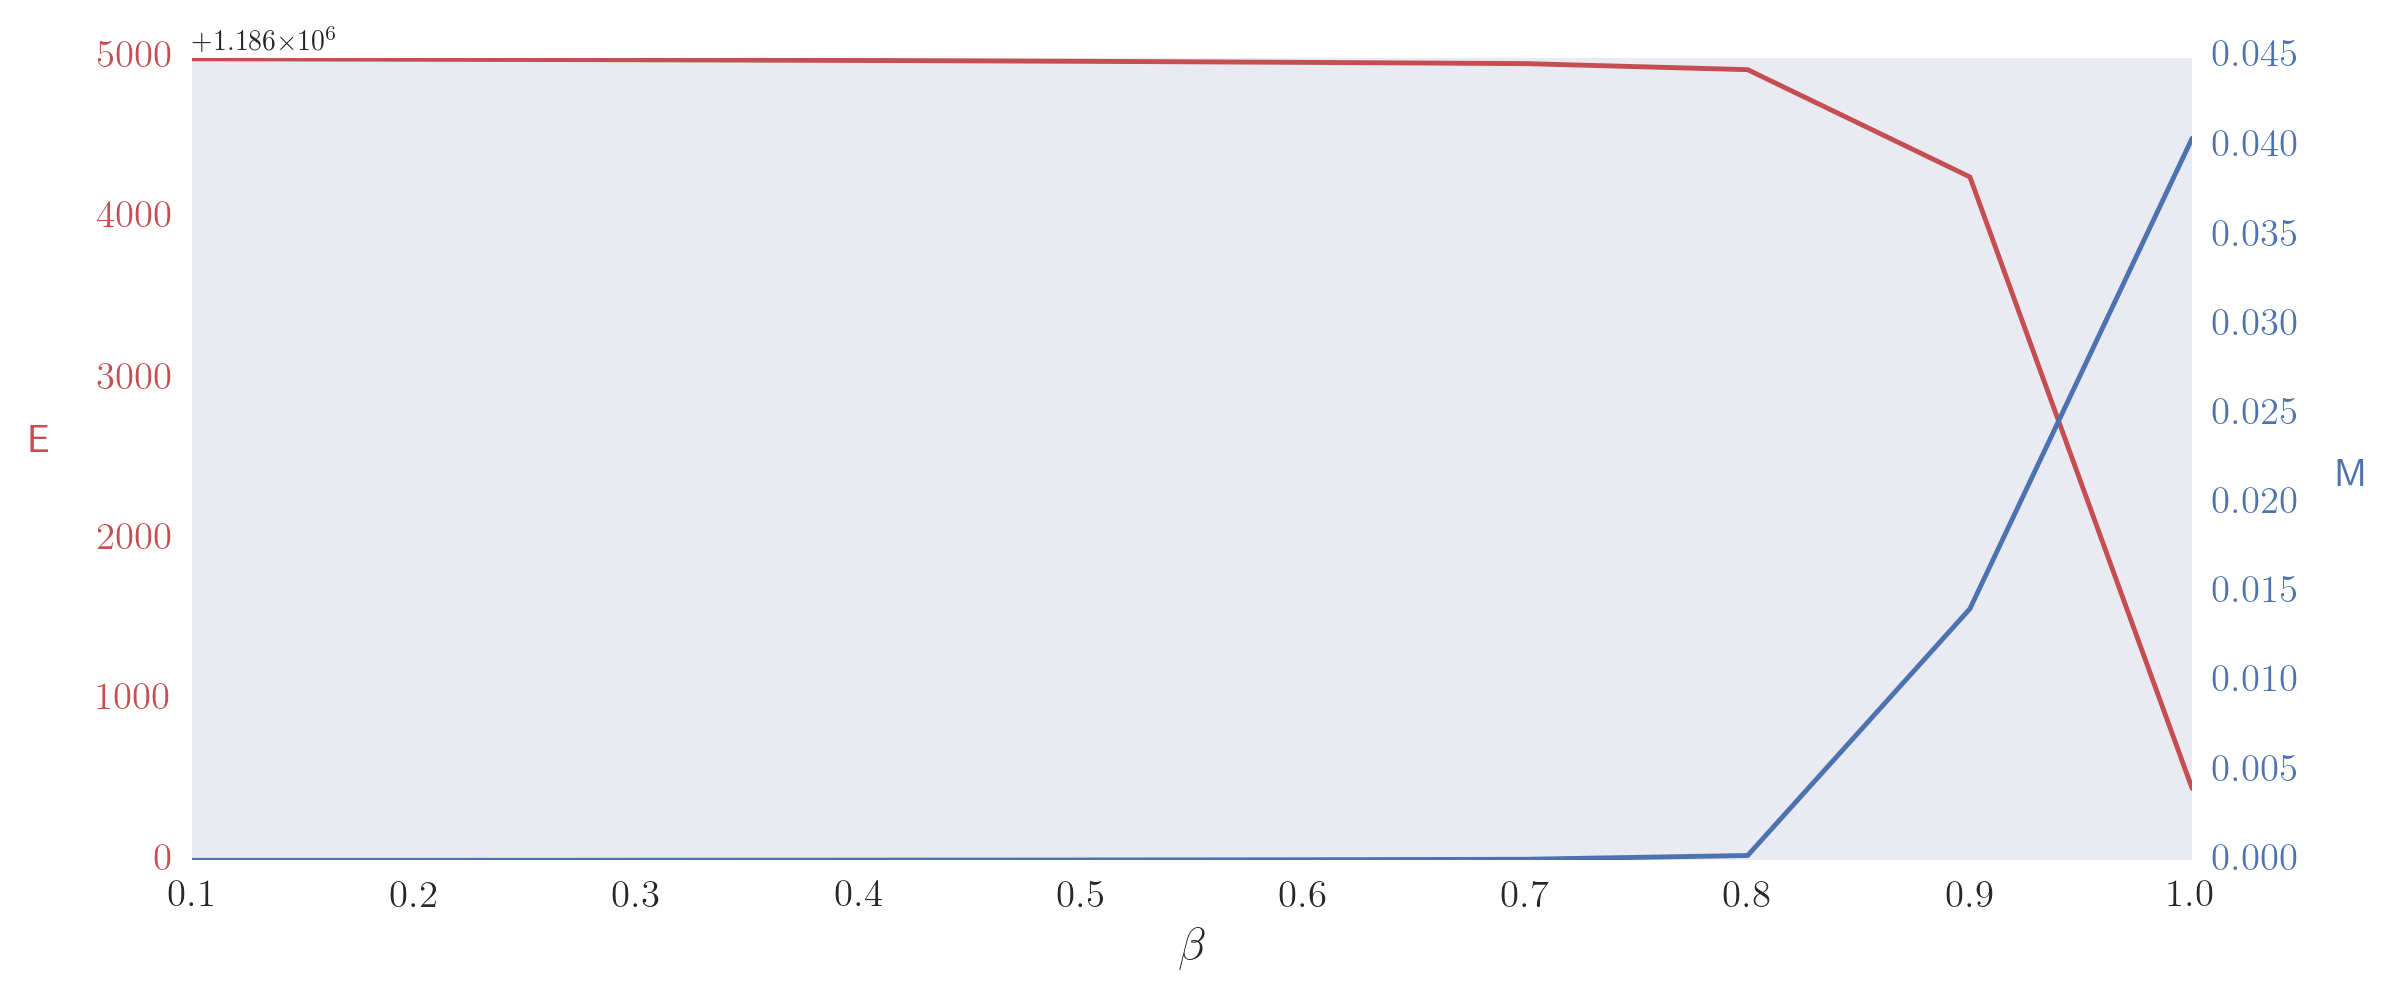
\includegraphics[width=\linewidth]{img/ising-energy-magnetization.png}
% }
% \caption{Energy (E) and magnetization (M) if the Ising spin model with
%   respect to the hyper-parameter $\beta$.}\label{snt:fig:ising-spin-em}
% \end{figure}

\begin{table}[h]
  \begin{center}
    \bgroup \setlength\tabcolsep{0.1\tabcolsep}\scriptsize
    \begin{tabular}{p{0.172\columnwidth} % first columm
        >{\centering\arraybackslash}p{0.06\columnwidth} % second columm
        *{9}{>{\centering\arraybackslash}p{0.07\columnwidth}} % next nine columns
        *{2}{>{\centering\arraybackslash}p{0.053\columnwidth}}} % last two columns
      \toprule
      \multirow{2}*{\bfseries Lexicon} & %
      \multirow{2}{0.06\columnwidth}{\bfseries \# of Terms} & %
      \multicolumn{3}{c}{\bfseries Positive Expressions} & %
      \multicolumn{3}{c}{\bfseries Negative Expressions} & %
      \multicolumn{3}{c}{\bfseries Neutral Terms} & %
      \multirow{2}{0.068\columnwidth}{\bfseries\centering Macro\newline \F{}} & %
      \multirow{2}{0.068\columnwidth}{\bfseries\centering Micro\newline \F{}}\\
      \cmidrule(lr){3-5}\cmidrule(lr){6-8}\cmidrule(lr){9-11}

      & & Precision & Recall & \F{} & %
      Precision & Recall & \F{} & %
      Precision & Recall & \F{} & & \\\midrule
      %% \multicolumn{9}{|c|}{\cellcolor{cellcolor}Existing Lexica}\\\hline

      % Class                     Precision              Recall                 F-score
      % positive                   0.770601             0.101975                 0.180115
      % negative                   0.567901             0.017139                 0.033273
      % neutral                    0.963176             0.999227                 0.980870
      % Macro-average              0.767226             0.372780                 0.398086
      % Micro-average              0.962404             0.962216                 0.962310

      \textsc{Seed Set} & 20 & \textbf{0.771} & 0.102 & 0.18 & %
      \textbf{0.568} & 0.017 & 0.033 & %
      0.963 & \textbf{0.999} & \textbf{0.981} & %
      0.398 & \textbf{0.962}\\

      % Class                     Precision              Recall                 F-score
      % positive                   0.646220             0.133510                 0.221299
      % negative                   0.565217             0.029061                 0.055280
      % neutral                    0.964071             0.998134                 0.980807
      % Macro-average              0.725169             0.386902                 0.419129
      % Micro-average              0.962261             0.962072                 0.962167

      TKM & 920 & 0.646 & \textbf{0.134} & \textbf{0.221} & %
      0.565 & \textbf{0.029} & \textbf{0.055} & %
      \textbf{0.964} & 0.998 & \textbf{0.981} & %
      \textbf{0.419} & \textbf{0.962}\\

      % Class                     Precision              Recall                 F-score
      % positive                   0.764317             0.102269                 0.180400
      % negative                   0.567901             0.017139                 0.033273
      % neutral                    0.963181             0.999199                 0.980860
      % Macro-average              0.765133             0.372869                 0.398178
      % Micro-average              0.962384             0.962196                 0.962290

      VEL & 60 & 0.764 & 0.102 & 0.18 & %
      \textbf{0.568} & 0.017 & 0.033 & %
      0.963 & 0.999 & 0.98 & %
      0.398 & \textbf{0.962}\\

      % Class                     Precision              Recall                 F-score
      % positive                   0.386437             0.105806                 0.166127
      % negative                   0.567901             0.017139                 0.033273
      % neutral                    0.963178             0.996092                 0.979359
      % Macro-average              0.639172             0.373012                 0.392920
      % Micro-average              0.959478             0.959290                 0.959384

      KIR & 320 & 0.386 & 0.106 & 0.166 & %
      \textbf{0.568} & 0.017 & 0.033 & %
      0.963 & 0.996 & 0.979 & %
      0.393 & 0.959\\

      % Class                     Precision              Recall                 F-score
      % positive                   0.679764             0.101975                 0.177345
      % negative                   0.567901             0.017139                 0.033273
      % neutral                    0.963162             0.998820                 0.980667
      % Macro-average              0.736942             0.372644                 0.397095
      % Micro-average              0.962013             0.961825                 0.961919

      SEV & 60 & 0.68 & 0.102 & 0.177 & %
      \textbf{0.568} & 0.017 & 0.033 & %
      0.963 & \textbf{0.999} & \textbf{0.981} & %
      0.397 & \textbf{0.962}\\

      TKM $\cap$ VEL $\cap$ SEV & 20 & \textbf{0.771} & 0.102 & 0.18 & %
      \textbf{0.568} & 0.017 & 0.033 & %
      0.963 & \textbf{0.999} & \textbf{0.981} & %
      0.398 & \textbf{0.962}\\

      % Class                     Precision              Recall                 F-score
      % positive                   0.592689             0.133805                 0.218322
      % negative                   0.565217             0.029061                 0.055280
      % neutral                    0.964063             0.997700                 0.980593
      % Macro-average              0.707323             0.386855                 0.418065
      % Micro-average              0.961850             0.961662                 0.961756

      TKM $\cup$ VEL $\cup$ SEV & 1,020 & 0.593 & \textbf{0.134} & 0.218  & %
      0.565 & \textbf{0.029} & \textbf{0.055} & %
      \textbf{0.964} & 0.998 & 0.98 & %
      0.418 & \textbf{0.962}\\\bottomrule
    \end{tabular}
    \egroup
    \caption{Evaluation of corpus-based approaches.\\ {\small TKM --
        \citet{Takamura:05}, VEL -- \citet{Velikovich:10}, KIR --
        \citet{Kiritchenko:14}, SEV -- \citet{Severyn:15}}}
    \label{snt-lex:tbl:corp-meth}
  \end{center}
\end{table}

The results of this evaluation are shown in
Table~\ref{snt-lex:tbl:corp-meth}.  This time, we can observe a clear
superiority of Takamura et al.'s method, which not only achieves the
best recall and \F{} in recognizing positive and negative items but
also attains the highest micro- and macro-averaged results for all
three polarity classes.
% As expected, the best precision in recognizing polar terms is achieved
% by the manually compiled seed set, whose micro-averaged \F{}-result,
% however, is still identical to the one shown by the method of
% \citet{Takamura:05}.
The size and scores of the other lexicons, however, are much smaller
than the cardinalities and results shown by Takamura et al.'s and
dictionary-based approaches.  Moreover, those polarity lists also show
absolutely identical scores for the negative expressions as the
original seed set.  Since these results were somewhat unexpected, we
decided to investigate the reasons for possible problems.  As it
turned out, the macro-averaged \F{}-values of the other methods were
rapidly going down on the held-out development set as the number of
their induced polar terms increased.  Since we considered the lexicon
size as one of the hyper-parameters of the tested approaches, we
rapidly stopped populating these lexicons when we noticed a decrease
in their results.  As a consequence, only the highest-ranked terms
(all of which had the positive polarity) were included in the final
lists.

A closer look at the data revealed that the positive bias of the
learned lexicons was mainly due to the ambiguity of the seed set:
While converting the original seed list of \citet{Turney:03} to
German, we translated the English word ``correct'' as ``richtig''.
This German word, however, also has another reading which means
\emph{real} (as in \emph{a real fact} or \emph{a real sports car}) and
which was much more frequent in the analyzed snapshot, also often
appearing in a negative context, e.g., ``ein richtiger
Bombenanschlag'' (\emph{a real bomb attack}) or ``ein richtiger
Terrorist'' (\emph{a real terrorist}).  As a consequence of this,
methods relying on distant supervision had to deal with an extremely
unbalanced training set (the automatically labeled corpus that we
obtained for the approach of \citet{Kiritchenko:14} using these seeds,
for instance, had 716,210 positive versus 92,592 negative training
instances).  We will investigate later in
Subsection~\ref{subsec:snt-lex:eoss} whether other seed sets could
provide a remedy to this problem.

\subsubsection{Lexicon Generation Using Neural Word Embeddings}

% \citet{Tang:14}

% \citet{Tang:14a}

% Similarly to \citet{Severyn:15a}, \citet{Vo:16} applied a deep
% learning approach learning two-dimensional embeddings (one dimension
% for the positive score and one dimension for the negative appraisal)

% \citet{Ren:16}

% A new family of lexicon induction methods builds on learned vector
% representations of words -- the neural word embeddings
% \cite{Mikolov:13}.

% Vector command:
% \begin{verbatim}
% Adjusted Potts' Tokenizer

% Sidarenka's Preprocessing (Smiley Replacement)

% word2vec -train tokens.tok -output vectors.txt -size 400 -window 5 -min-count 4

% Possible Improvements:

% * use task specific vectors;

% * decide what to do with smileys during evaluation;

% * explore different cardinalities (not just 40-s bins);
% \end{verbatim}

% % k-NN: k^2 / \sum d_{ij}

% The results of these methods are shown in Table~\ref{snt-lex:tbl:nwe-methods}.

% \begin{table}[h]
%   \begin{center}
%     \bgroup \setlength\tabcolsep{0.1\tabcolsep}\scriptsize
%     \begin{tabular}{p{0.1\columnwidth} % first columm
%         *{9}{>{\centering\arraybackslash}p{0.078\columnwidth}} % next nine columns
%         *{2}{>{\centering\arraybackslash}p{0.078\columnwidth}}} % last two columns
%       \toprule
%           \multirow{2}*{\bfseries Lexicon} & %
%           \multicolumn{3}{c}{\bfseries Positive Expressions} & %
%           \multicolumn{3}{c}{\bfseries Negative Expressions} & %
%           \multicolumn{3}{c}{\bfseries Neutral Terms} & %
%           \multirow{2}{0.068\columnwidth}{\bfseries\centering Macro\newline \F{}} & %
%           \multirow{2}{0.068\columnwidth}{\bfseries\centering Micro\newline \F{}}\\
%           \cmidrule(lr){2-4}\cmidrule(lr){5-7}\cmidrule(lr){8-10}

%           & Precision & Recall & \F{} & %
%           Precision & Recall & \F{} & %
%           Precision & Recall & \F{} & & \\\midrule

%           % cardinality 160
%           NC & 75.7\stddev{23.8} & 9.1\stddev{5.7} & 15.8\stddev{8.8} & %
%           24.4\stddev{41.8} & 1\stddev{1.8} & 1.9\stddev{3.4} & %
%           96.3\stddev{0.8} & \textbf{99.9}\stddev{0.1} & \textbf{98.1}\stddev{0.4} & %
%           38.6\stddev{3.2} & \textbf{96.2}\stddev{0.8}\\

%           % cardinality 40
%           KNN & \textbf{75.8}\stddev{23.8} & 9.1\stddev{5.7} & 15.8\stddev{8.8} & %
%           23.4\stddev{40.6} & 1\stddev{1.8} & 1.8\stddev{3.4} & %
%           96.3\stddev{0.8} & \textbf{99.9}\stddev{0.1} & \textbf{98.1}\stddev{0.4} & %
%           38.6\stddev{3.2} & \textbf{96.2}\stddev{0.8}\\

%           % cardinality 160
%           PCA & 40.4\stddev{14.6} & \textbf{13.4}\stddev{5.8} & \textbf{19.5}\stddev{7.3} & %
%           24.4\stddev{41.8} & 1\stddev{1.8} & 1.9\stddev{3.4} & %
%           \textbf{96.4}\stddev{0.8} & 99.6\stddev{0.2} & 97.9\stddev{0.4} & %
%           39.8\stddev{2.7} & 95.9\stddev{0.8}\\

%           % cardinality 160
%           LP & \textbf{75.8}\stddev{23.8} & 9.1\stddev{5.7} & 15.8\stddev{8.8} & %
%           \textbf{29.4}\stddev{20.3} & \textbf{5.6}\stddev{4.5} & \textbf{9.2}\stddev{6.9} & %
%           \textbf{96.4}\stddev{0.8} & 99.8\stddev{0.1} & 98\stddev{0.4} & %
%           \textbf{41}\stddev{3.9} & 96.1\stddev{0.8}\\
%           \bottomrule
%     \end{tabular}
%     \egroup
%     \caption{Evaluation of embedding-based approaches.\\ {\small (NC
%         -- nearest centroids, KNN -- k-nearest neighbors, PCA --
%         principal component analysis, LP -- linear projection)}}
%     \label{snt-lex:tbl:nwe-methods}
%   \end{center}
% \end{table}

\subsection{Effect of Seed Sets}\label{subsec:snt-lex:eoss}

An important factor which could significantly affect the quality of
the resulting polarity lists was the set of the seed terms that we
used to initialize the polarity scores of the evaluated methods.  In
order to estimate the impact of this setting on the final scores, we
re-run our experiments using the seed lists proposed by \citet{Hu:04},
\citet{Kim:04}, \citet{Esuli:06c}, and \citet{Remus:10}.  In the cases
where theses resources were missing the neutral class, we explicitly
added a set of neutral terms proportional to the size of the polar
categories.  Moreover, since \citet{Hu:04} only partially specified
their seed list in the original paper, and \citet{Kim:04} did not
provide any examples of their seed terms at all, we filled the missing
entries in these lists with common polar German words that we came up
with in order to match the reported size of these seed sets.  Finally,
since the set of neutral terms from the polarity list of
\citet{Esuli:06c} comprised 4,122 words---the authors considered as
neutral all terms from the General Inquirer lexicon \cite{Stone:66}
which were not marked there as either positive or negative and did not
appear in the seed list of \citet{Turney:03}---and was therefore
tedious to translate manually, we automatically obtained translations
for these terms using the publicly available online dictionary
\texttt{dict.cc}\footnote{\url{http://www.dict.cc}} and taking the
first suggested German translation for each of the neutral
entries.\footnote{We also tried to use all possible translations of
  the original terms, but it lead to a considerable boost in the
  number of neutral items (45,252 words) and resulted in a substantial
  decrease of the final system scores.} A short statistics on the
cardinality and composition of the resulting seed sets is presented in
Table~\ref{snt-lex:tbl:alt-seed-sets}.

\begin{table}[h]
  \begin{center}
    \bgroup \setlength\tabcolsep{0.1\tabcolsep}\scriptsize
    \begin{tabular}{ %
        >{\centering\arraybackslash}p{0.2\columnwidth} % first columm
        *{4}{>{\centering\arraybackslash}p{0.2\columnwidth}}} % next four columns
      \toprule
      {\bfseries Seed Set} & %
      {\bfseries Cardinality} & %
      {\bfseries Parts of Speech} & %
      {\bfseries Examples} & %
      {\bfseries Comments}\\
      \midrule
      \citet{Hu:04} & 14 positive, 15 negative, and 10 neutral terms & adjectives %
      & {{\itshape fantastisch, lieb, sympathisch, %
          b\"ose, dumm, schwierig}} & polar terms translated from the original paper %
      \cite{Hu:04}; neutral terms added by us;\\
      \citet{Kim:04} & 60 positive, 60 negative, and 60 neutral terms & any & %
      {\itshape fabelhaft, Hoffnung, lieben, h\"asslich, Missbrauch, t\"oten} %
      & devised by us so as to match the cardinality of the original set with %
      neutral terms added extra;\\
      \citet{Esuli:06c} & 16 positive, 35 negative, and 4,122 neutral terms & %
      any & {\itshape angenehm, ausgezeichnet, freundlich, %
        arm, bedauernswert, d\"urftig} & polar terms translated from the seed %
      set of \citet{Turney:03}; neutral terms automatically translated from %
      objective entries in the General Inquirer lexicon \cite{Stone:66};\\
      \citet{Remus:10} & 12 positive, 12 negative, and 10 neutral terms & %
      adjectives & {\itshape gut, sch\"on, richtig, %
        schlecht, unsch\"on, falsch} & %
      polar terms translated from the seed set of \citet{Turney:03}; %
      neutral terms added by us.\\
      \\\bottomrule
    \end{tabular}
    \egroup
    \caption{Cardinality and composition of the alternative polarity lists.\\
      (all cardinalities are given with respect to the resulting
      German translations)}
    \label{snt-lex:tbl:alt-seed-sets}
  \end{center}
\end{table}

The updated results for the dictionary-based approaches with these
alternative seed sets are shown in
Figure~\ref{snt:fig:sent-dict-lex-alt-seeds}.  This time, we again can
notice superior scores achieved by the method of
\citet{Blair-Goldensohn:08}, which not only outperforms other systems
on average but also seems to be less susceptible to the varying
quality and size of the different seed lists.  The remaining methods
typically achieve their best macro-averaged \F{}-results with either
of the two top-performing seed lists: the seed set of \citet{Kim:04}
or the seed set of \citet{Esuli:06c}.  The former option works best
for the label-propagation approach \citet{Rao:09} and the random walk
algorithm of \citet{Awadallah:10}.  Moreover, the results shown by the
min-cut system \cite{Rao:09} and the original method of \citet{Kim:04}
when used with this seed set are only slightly lower than their
respective scores achieved with the best possible configuration---the
seed list of \citet{Turney:02}.  The latter option---the seed set of
\citet{Esuli:06c}---shows best results for the approaches of
\citet{Hu:04} and the \textsc{SentiWordNet} method of \citet{Esuli:06c}.

\begin{figure}[hbtp!]
  \centering
  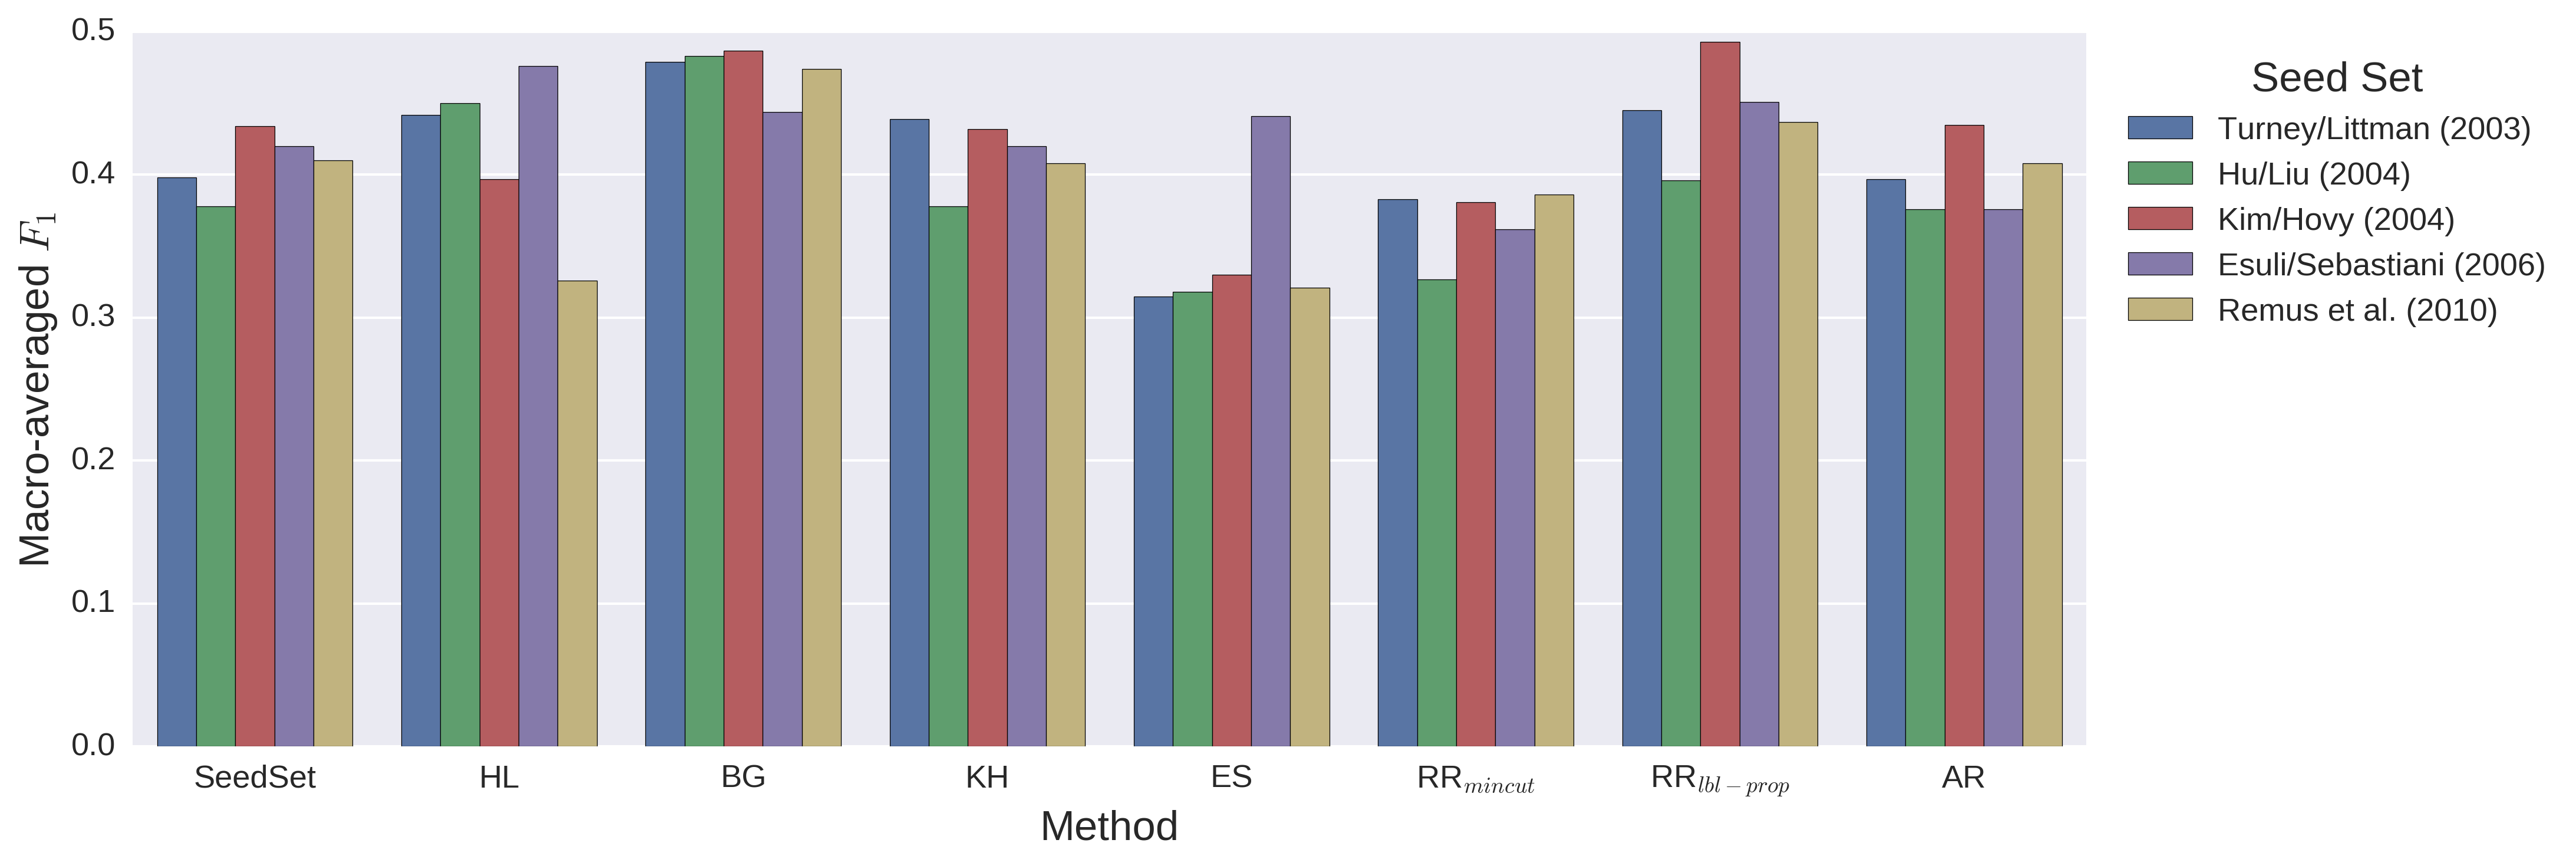
\includegraphics[height=12em,width=\linewidth]{%
    img/sentilex-dict-alt-seed-sets.png}
  \caption{Macro-averaged \F{}-scores of the dictionary-based approaches
    with different seed sets.}\label{snt:fig:sent-dict-lex-alt-seeds}
\end{figure}

A slightly different situation is observed for the corpus-based
approaches as shown in Figure~\ref{snt:fig:sent-crp-lex-alt-seeds}.
Except for the method of \citet{Takamura:05}, which achieves its best
result with the seed set of \citet{Hu:04}, all three remaining
methods---\citet{Velikovich:10}, \citet{Kiritchenko:14}, and
\citet{Severyn:15}---show very similar (though not identical) scores
to the ones reached by the non-expanded seed sets.  The primary reason
for this is again the ambiguity of the translated seeds, which causes
a rapid decrease of the lexicon quality and, consequently, an early
stopping of the expansion.

\begin{figure}[hbtp!]
  \centering
  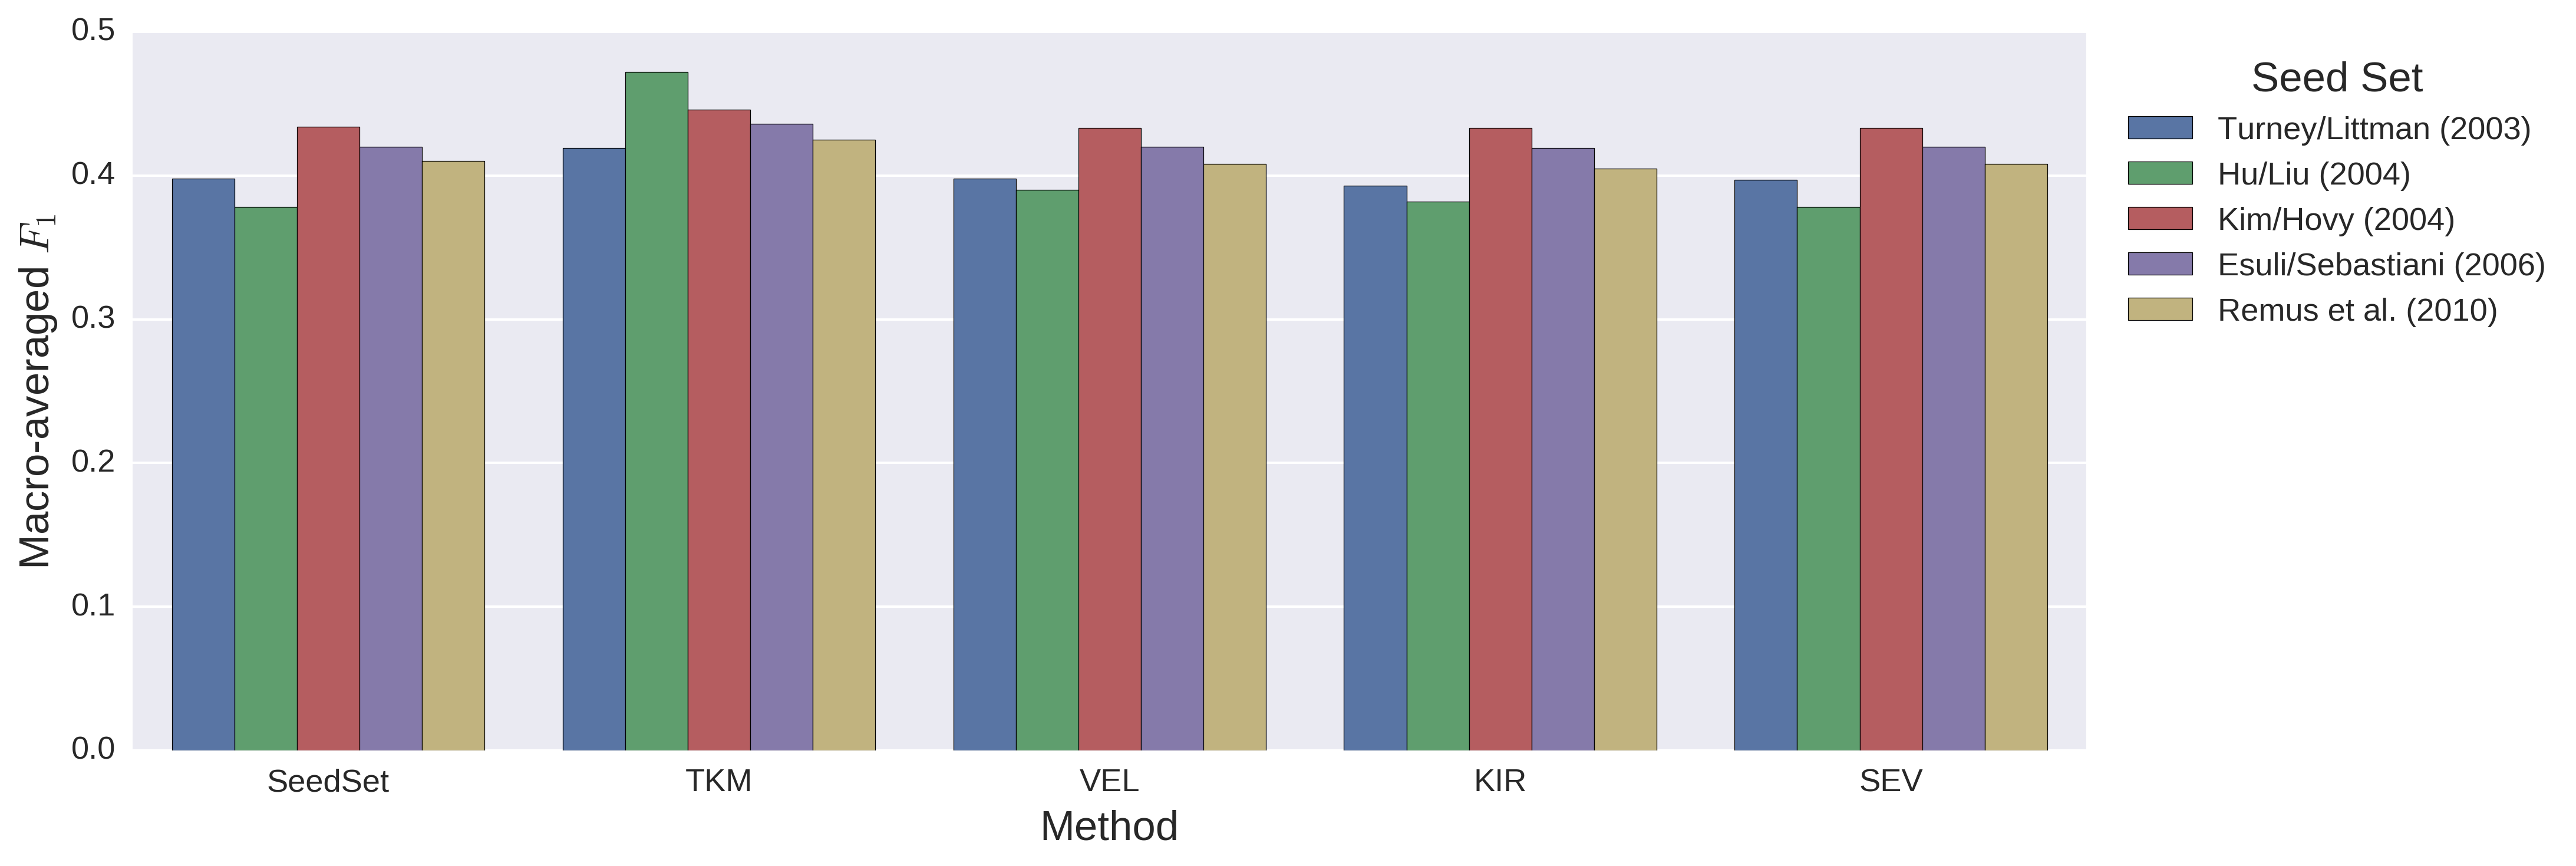
\includegraphics[height=12em,width=\linewidth]{%
    img/sentilex-crp-alt-seed-sets.png}
  \caption{Macro-averaged \F{}-scores of the corpus-based approaches
  with different seed sets.}\label{snt:fig:sent-crp-lex-alt-seeds}
\end{figure}

% For convenience, we will summarize the results of three top-performing
% configurations---the methods of \citet{Blair-Goldensohn:08},
% \citet{Kim:04,Kim:06}, and the label-propagation approach of
% \citet{Rao:09} used in combination with the initial seed sed of
% \citet{Kim:04}---in Table~\ref{snt-lex:tbl:lex-kh-seedset} and use
% these results as baselines in our later experiments.

% \begin{table}[h]
%   \begin{center}
%     \bgroup \setlength\tabcolsep{0.1\tabcolsep}\scriptsize
%     \begin{tabular}{p{0.1\columnwidth} % first columm
%         *{9}{>{\centering\arraybackslash}p{0.078\columnwidth}} % next nine columns
%         *{2}{>{\centering\arraybackslash}p{0.078\columnwidth}}} % last two columns
%       \toprule
%           \multirow{2}*{\bfseries Lexicon} & %
%           \multicolumn{3}{c}{\bfseries Positive Expressions} & %
%           \multicolumn{3}{c}{\bfseries Negative Expressions} & %
%           \multicolumn{3}{c}{\bfseries Neutral Terms} & %
%           \multirow{2}{0.068\columnwidth}{\bfseries\centering Macro\newline \F{}} & %
%           \multirow{2}{0.068\columnwidth}{\bfseries\centering Micro\newline \F{}}\\
%           \cmidrule(lr){2-4}\cmidrule(lr){5-7}\cmidrule(lr){8-10}

%           & Precision & Recall & \F{} & %
%           Precision & Recall & \F{} & %
%           Precision & Recall & \F{} & & \\\midrule

%           BG & 22.7\stddev{6.5} & \textbf{29.9}\stddev{8.4} & 25.4\stddev{6.7} & %
%           17.1\stddev{7.4} & \textbf{16.9}\stddev{7.2} & \textbf{16.6}\stddev{6.7} & %
%           \textbf{97}\stddev{0.6} & 96.4\stddev{0.6} & 96.7\stddev{0.5} & %
%           46.3\stddev{3.5} & 93.5\stddev{0.9}\\

%           KH & 51.6\stddev{12.4} & 21.7\stddev{7.2} & \textbf{29.9}\stddev{8.1} & %
%           38.9\stddev{24.7} & 7.5\stddev{4.9} & 12.2\stddev{7.8} & %
%           96.7\stddev{0.7} & \textbf{99.4}\stddev{0.2} & \textbf{98}\stddev{0.4} & %
%           \textbf{46.7}\stddev{3.9} & \textbf{96}\stddev{0.7}\\

%           RR$_{\textrm{lbl-prop}}$ & \textbf{52.9}\stddev{15.2} & 18.4\stddev{6.5} & 26.7\stddev{8.2} & %
%           \textbf{42.8}\stddev{29.7} & 8.9\stddev{5.8} & 14.1\stddev{8.8} & %
%           96.6\stddev{0.7} & \textbf{99.4}\stddev{0.3} & \textbf{98}\stddev{0.4} & %
%           46.3\stddev{4.3} & \textbf{96}\stddev{0.8}\\
%           \bottomrule
%     \end{tabular}
%     \egroup
%     \caption{Results of the top-scoring dictionary-based approaches
%       with the best observed seed set configuration. {\small (BG --
%         \citet{Blair-Goldensohn:08}, KH -- \citet{Kim:04,Kim:06}, RR
%         -- \citet{Rao:09})}}
%     \label{snt-lex:tbl:lex-kh-seedset}
%   \end{center}
% \end{table}

\subsection{Analysis of Entries}\label{subsec:snt-lex:aoe}

Besides investigating the effects of different hyper-parameters and
seed sets, we also decided to have a closer look at the actual results
produced by the tested methods.  For this purpose, we extracted ten
highest scored entries (not counting the seed terms) from each
dictionary-based automatic lexicon and summarized them in
Table~\ref{tbl:snt-lex:dict:top-10}.

\begin{table}[h]
  \begin{center}
    \bgroup \setlength\tabcolsep{0.03\tabcolsep}\scriptsize
    \begin{tabular}{%
        >{\centering\arraybackslash}p{0.07\columnwidth} % first columm
        *{6}{>{\centering\arraybackslash}p{0.155\columnwidth}}} % last two columns
      \toprule
      \textbf{Rank} & %
      \textbf{HL} & \textbf{BG} & \textbf{KH} & %
      \textbf{ES} & \textbf{RR}$^{**}_{\textrm{mincut}}$ & %
      \textbf{RR}$_{\textrm{lbl-prop}}$\\\midrule
      1 & \ttranslate{perfekt}{perfect} & %
      \ttranslate{flei\ss{}ig}{diligent} &%
      \ttranslate{anr\"uchig}{indecent} &%
      \ttranslate{namenlos}{nameless} &%
      \ttranslate{planieren}{to plane} &%
      \ttranslate{prunkvoll}{splendid}\\

      2 & \ttranslate{musterg\"ultig}{immaculate} & %
      \ttranslate{b\"ose}{evil} &%
      \ttranslate{unecht}{artificial} &%
      \ttranslate{ruhelos}{restless} &%
      \ttranslate{Erdschicht}{stratum} &%
      \ttranslate{sinnlich}{sensual}\\


      3 & \ttranslate{vorbildlich}{commendable} & %
      \ttranslate{beispielhaft}{exemplary} &%
      \ttranslate{irregul\"ar}{irregular} &%
      \ttranslate{unbewaffnet}{unarmed} &%
      \ttranslate{gefallen}{please} &%
      \ttranslate{pomp\"os}{ostentatious}\\

      4 & \ttranslate{beispielhaft}{exemplary} & %
      \ttranslate{edel}{noble} &%
      \ttranslate{drittklassig}{third-class} &%
      \ttranslate{interesselos}{indifferent} &%
      \ttranslate{Zeiteinheit}{time unit} &%
      \ttranslate{unappetitlich}{unsavory}\\

      5 & \ttranslate{exzellent}{excellent} & %
      \ttranslate{t\"uchtig}{proficient} &%
      \ttranslate{sinnlich}{sensual} &%
      \ttranslate{reizlos}{unattractive} &%
      \ttranslate{Derivat}{derivate} &%
      \ttranslate{befehlsgem\"a\ss{}}{as ordered}\\

      6 & \ttranslate{exzeptionell}{exceptional} & %
      \ttranslate{emsig}{busy} &%
      \ttranslate{unprofessionell}{unprofessional} &%
      \ttranslate{w\"urdelos}{undignified} &%
      \ttranslate{Oberfl\"ache}{surface} &%
      \ttranslate{vierschr\"otig}{beefy}\\

      7 & \ttranslate{au\ss{}ergew\"ohnlich}{extraordinary} & %
      \ttranslate{eifrig}{eager} &%
      \ttranslate{abgeschlagen}{exhausted} &%
      \ttranslate{absichtslos}{unintentional} &%
      \ttranslate{Essbesteck}{cutlery} &%
      \ttranslate{regelgem\"a\ss}{regularly}\\

      8 & \ttranslate{au\ss{}erordentlich}{exceptionally} & %
      \ttranslate{arbeitsam}{hardworking} &%
      \ttranslate{gef\"allig}{pleasing} &%
      \ttranslate{ereignislos}{uneventful} &%
      \ttranslate{abl\"osen}{to displace} &%
      \ttranslate{wahrheitsgem\"a\ss}{true}\\

      9 & \ttranslate{viertklassig}{fourth-class} & %
      \ttranslate{musterg\"ultig}{exemplary} &%
      \ttranslate{musterg\"ultig}{exemplary} &%
      \ttranslate{regellos}{irregular} &%
      \ttranslate{Musikveranstaltung}{music event} &%
      \ttranslate{fettig}{greasy}\\

      10 & \ttranslate{sinnreich}{ingenious} & %
      \ttranslate{vorbildlich}{commendable} &%
      \ttranslate{unrecht}{wrong} &%
      \ttranslate{fehlerfrei}{accurate} &%
      \ttranslate{Gebrechen}{afflictions} &%
      \ttranslate{lumpig}{shabby}\\\bottomrule
    \end{tabular}
    \egroup
    \caption{Top ten polar terms produced by the dictionary-based methods.\\
      {\small ** -- the min-cut method of \citet{Rao:09} returns an
        unsorted set}}
    \label{tbl:snt-lex:dict:top-10}
  \end{center}
\end{table}

As can be seen from the table, the approaches by \citet{Hu:04},
\citet{Blair-Goldensohn:08}, \citet{Kim:04}, as well as the
label-propagation algorithm by \citet{Rao:09} produce almost perfect
polarity lists.  The \textsc{SentiWordNet} approach by \citet{Esuli:06c},
however, already features some spurious terms (e.g., ``absichtslos''
\emph{unintentional}) among its top-scored entries.  Finally, the
min-cut approach by \citet{Rao:09} returns a set of mainly objective
terms, which, however, is rather due to the fact that this method
performs a cluster-like partitioning of the lexical graph and does not
rank words assigned to a cluster.

An opposite situation is observed for the corpus-based systems as
shown in Table~\ref{tbl:snt-lex:crp:top-10}: The top-scoring polarity
lists returned by these approaches not only include many apparently
objective terms but are also difficult to interpret in general, as
they contain a substantial number of slang and advertising terms
(e.g., ``BMKS65'', ``\#gameinsight'', ``\#androidgames'' etc.).  This
again supports the hypothesis that an extreme noisiness of the input
domain might pose considerable difficulties to corpus-based
approaches.

\begin{table}[h]
  \begin{center}
    \bgroup \setlength\tabcolsep{0.03\tabcolsep}\scriptsize
    \begin{tabular}{%
        >{\centering\arraybackslash}p{0.07\columnwidth} % first columm
        *{4}{>{\centering\arraybackslash}p{0.232\columnwidth}}} % last two columns
      \toprule
      \textbf{Rank} & %
      \textbf{TKM} & \textbf{VEL} & \textbf{KIR} & %
      \textbf{SEV} \\\midrule
      1 & \ttranslate{Stockfotos}{stock photos} &%
      \ttranslate{Wahl\-kampf\-ge\-schenk}{election gift} &%
      \ttranslate{Suchmaschinen}{search engines} &%
      \ttranslate{Scherwey}{Scherwey}\\

      2 & \ttranslate{BMKS65}{BMKS65} &%
      \ttranslate{Or\-dens\-ge\-schich\-te}{order history} &%
      \ttranslate{\#gameinsight}{\#gameinsight} &%
      \ttranslate{krebsen}{to crawl}\\

      3 & \ttranslate{Ziya}{Ziya} &%
      \ttranslate{Indologica}{Indologica} &%
      \ttranslate{\#androidgames}{\#androidgames} &%
      \ttranslate{kaschieren}{to conceal}\\

      4 & \ttranslate{Shoafoundation}{shoah found.} &%
      \ttranslate{Indologie}{Indology} &%
      \ttranslate{Selamat}{selamat} &%
      \ttranslate{Davis}{Davis}\\

      5 & \ttranslate{T1199}{T1199} &%
      \ttranslate{Energieverbrauch}{energy consumption} &%
      \ttranslate{Pagi}{Pagi} &%
      \ttranslate{\#Klassiker}{\#classics}\\

      6 & \ttranslate{Emilay55}{Emilay55} &%
      \ttranslate{Schimmelbildung}{mold formation} &%
      \ttranslate{\#Sparwelt}{\#savingsworld} &%
      \ttranslate{Nationalismus}{nationalism}\\

      7 & \ttranslate{Eneramo}{Eneramo} &%
      \ttranslate{Hygiene}{hygiene} &%
      \ttranslate{\#Seittest}{\#Seittest} &%
      \ttranslate{Kraftstoff}{fuel}\\

      8 & \ttranslate{GotzeID}{GotzeID} &%
      \ttranslate{wasserd}{waterp} &%
      \ttranslate{Gameinsight}{Gameinsight} &%
      \ttranslate{inaktiv}{idle}\\

      9 & \ttranslate{BSH65}{BSH65} &%
      \ttranslate{heizkostensparen}{saving heating costs} &%
      \ttranslate{\#ipadgames}{\#ipadgames} &%
      \ttranslate{8DD}{8DD}\\

      10 & \ttranslate{Saymak.}{Saymak.} &%
      \ttranslate{Re\-fe\-renz\-ar\-chi\-tek\-tu\-ren}{reference architectures} &%
      \ttranslate{Fitnesstraining}{fitness training} &%
      \ttranslate{Mailadresse}{mail address}\\\bottomrule
    \end{tabular}
    \egroup
    \caption{Top ten polar terms produced by the corpus-based methods.}
    \label{tbl:snt-lex:crp:top-10}
  \end{center}
\end{table}

\subsection{Discussion}

In general, as we can see from the results, all systems tested in this
section performed notably worse than reported in their original
papers.  We can explain this divergence by the following four reasons:
\begin{enumerate}[1\upshape)]
\item the evaluation metrics that we applied in our experiments were
  considerably different from the testing methods used in the previous
  works (we estimated the results on a real-life corpus, counting
  every false positive and false negative match separately, whereas
  the English approaches typically evaluated their results on the
  intersection with the General Inquirer Lexicon \cite{Stone:66},
  omitting false positive matches and therefore artifically boosting
  their scores);
\item both the domain and the language that we addressed in this
  section were apparently more challenging than the standard English
  form for which most of these methods had been developed;
\item the notion of the synonymous relations used for the
  dictionary-based approaches and the set of the initial seed terms
  used by all methods could differ from the original settings of the
  evaluated algorithms;
\item finally, the underlying lexical taxonomy (\textsc{GermaNet}) and
  the snapshot corpus were different from the resources that were
  originally used for training the presented methods.
\end{enumerate}


% Since \textsc{GermaNet}, however, is significantly different from its
% English counterpart, both quantitatively and qualitatively, we should
% first present some key statistics (shown in
% Table~\ref{snt-lex:tbl:germanet-wordnet}) and visualize the synset
% graphs (demonstrated in Figures~\ref{snt-lex:fig:germanet}
% and~\ref{snt-lex:fig:wordnet}) of these lexical databases.

% \begin{table}[h]
%   \begin{center}
%     \bgroup \setlength\tabcolsep{0.1\tabcolsep}\scriptsize \small
%     \begin{tabular}{p{0.15\textwidth} % first columm
%         *{8}{>{\centering\arraybackslash}m{0.085\textwidth}}} % next nine columns
%       \toprule
%       & \multicolumn{2}{c}{\bfseries Noun} & %
%       \multicolumn{2}{c}{\bfseries Verb} & %
%       \multicolumn{2}{c}{\bfseries Adjective} & & \\
%       \multirow{-2}{0.12\columnwidth}{\centering\bfseries Resource} & %
%       Words & Synsets & Words & Synsets & Words & Synsets & %
%       \multirow{-2}{0.085\columnwidth}{\centering\scriptsize\bfseries{}Hy\-pon.\newline{}Rels} & %
%       \multirow{-2}{0.085\columnwidth}{\centering\scriptsize\bfseries{}Anto\-n.\newline{}Rels}\\
%       \midrule

%       \textsc{GermaNet} & 85,662 & 71,575 & 9,340 & 11,026 & 12,890 & 10,645 & %
%       97,712 & 1,741\\
%       \textsc{WordNet}  & 117,798 & 82,115 & 11,529 & 13,767 & 21,479 & 18,156 & %
%       95,322 & 7,394\\
%       \bottomrule
%     \end{tabular}
%     \egroup
%     \caption{Key statistics on \textsc{GermaNet} and
%       \textsc{WordNet}.}
%     \label{snt-lex:tbl:germanet-wordnet}
%   \end{center}
% \end{table}

% \begin{figure*}[htbp!]
% {
% \centering
% \begin{subfigure}{.5\textwidth}
%   \centering
%   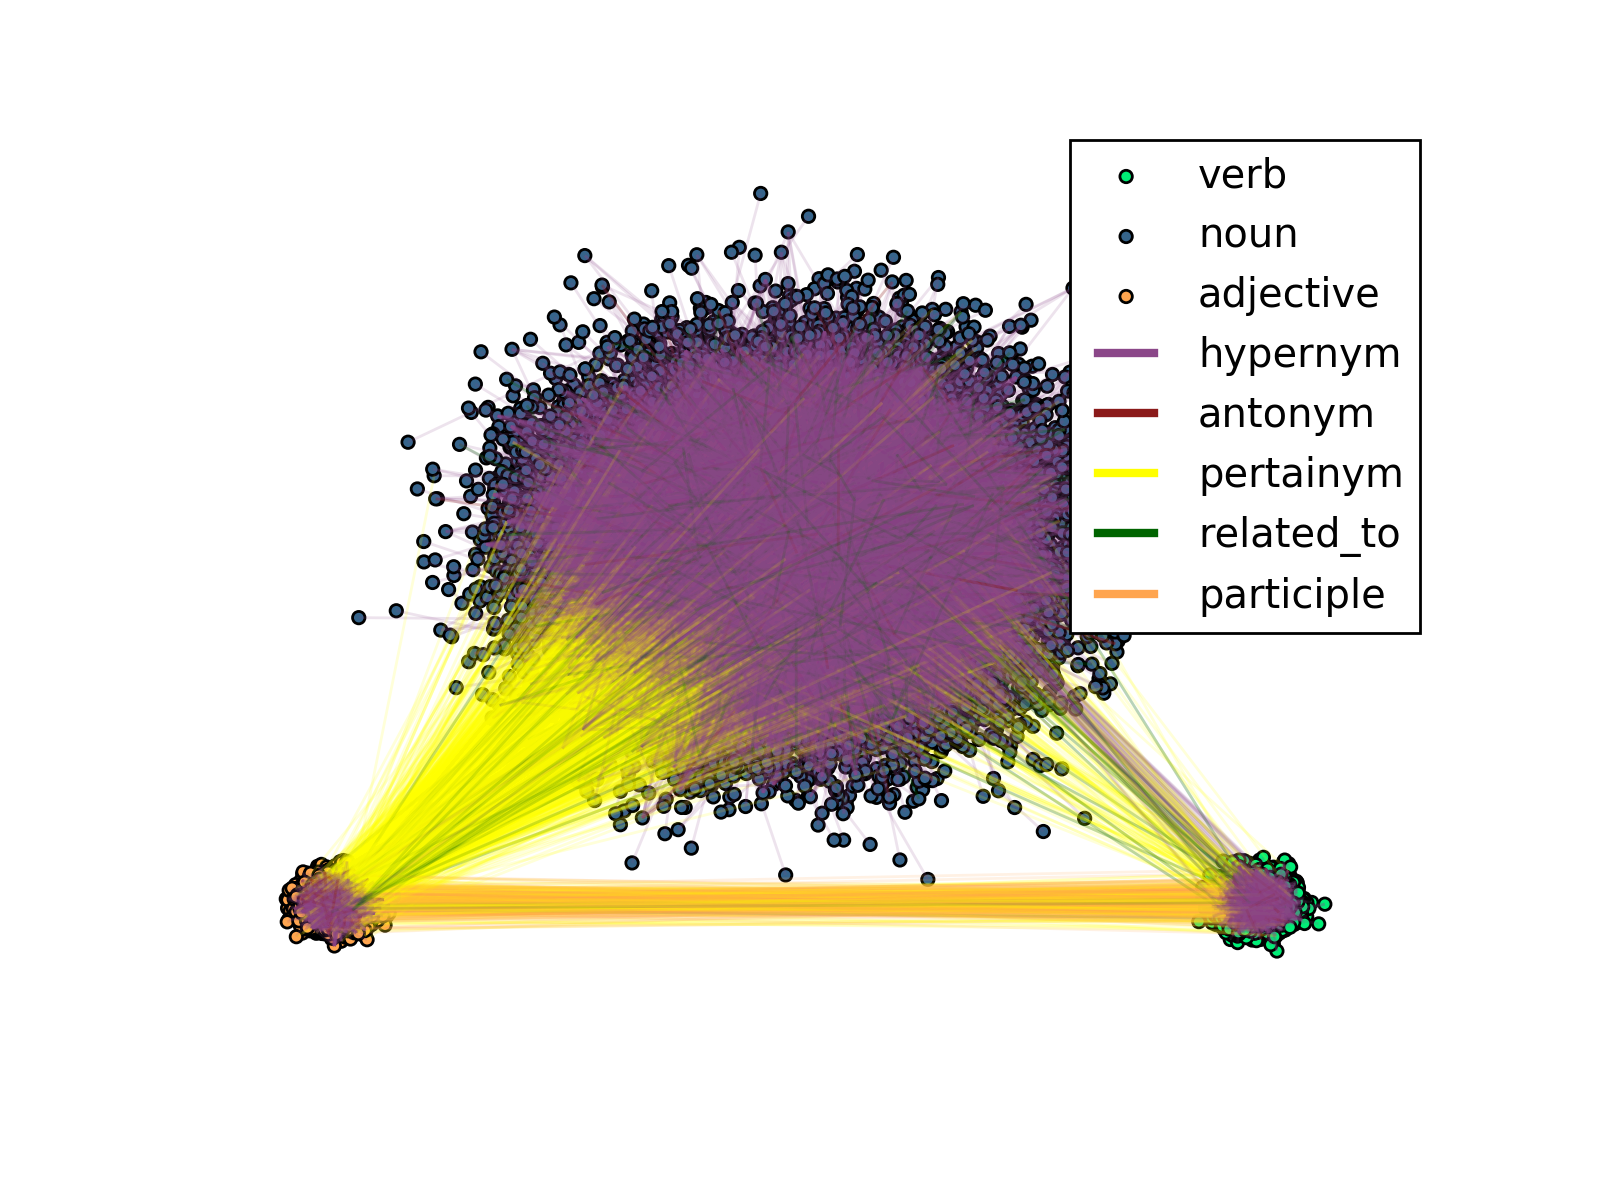
\includegraphics[width=\linewidth]{img/germanet.png}
%   \caption{\textsc{GermaNet}}\label{snt-lex:fig:germanet}
% \end{subfigure}%
% \begin{subfigure}{.5\textwidth}
%   \centering
%   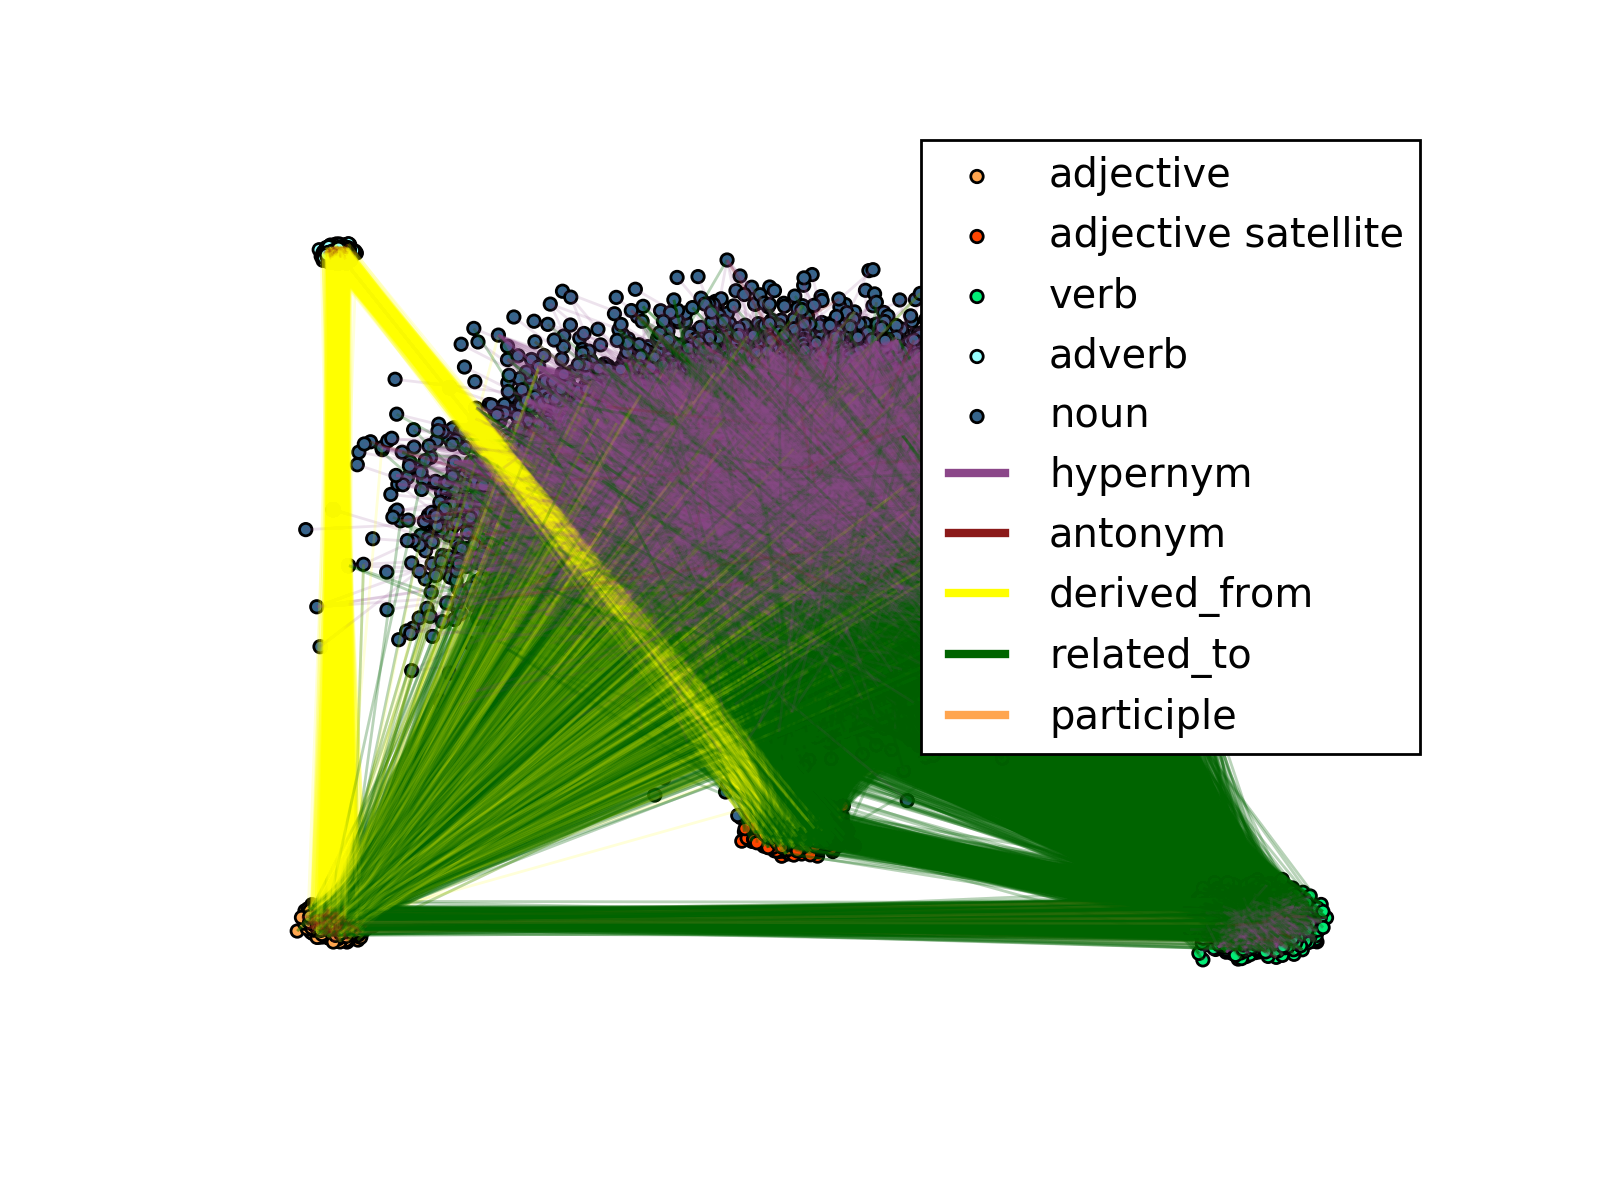
\includegraphics[width=\linewidth]{img/wordnet.png}
%   \caption{\textsc{WordNet}}\label{snt-lex:fig:wordnet}
% \end{subfigure}
% }
% \caption{Graphical visualization of \textsc{GermaNet} and
%       \textsc{WordNet}.}\label{snt:fig:crp-sent-emo-distr}
% \end{figure*}

% As can be seen from the table, \textsc{GermaNet} has significantly
% fewer words and synsets for all common parts of speech with the
% largest gaps observed for nouns and adjectives.  Moreover, as shown in
% Figures~\ref{snt-lex:fig:germanet} and~\ref{snt-lex:fig:wordnet}, such
% PoS-classes as adverbs and adjective satellites are completely missing
% in the German resource.  The reason for this is that the form (and
% meaning) of most German adverbs typically coincides with that of the
% adjectives; therefore, both categories are treated in the same way,
% being represented through the adjectival synsets.

% A slightly different situation can be observed for the semantic links
% (relations) between the synsets: here, \textsc{GermaNet} features
% almost 2,500 more hypernym-hyponym pairs than the English resource,
% whereas the number of antonyms is more than four times less than in
% \textsc{WordNet}.

% An especially interesting pattern, however, appears with the relations
% connecting different parts of speech: As can be seen from the figures,
% the strongest inter-PoS connections in \textsc{GermaNet} are the
% pertainym links between the adjectives and nouns and the participle
% edges between the adjectives and verbs.  The interlinks between the
% nouns and verbs, however, are both much fewer in number and more
% diverse in their nature.  This situation is different in
% \textsc{WordNet} where the prevailing majority of the
% inter-part-of-speech connections are represented through the
% \texttt{related\_to} (especially between the nouns, adjective
% satellites, verbs, and verbs and adjectives) and
% \texttt{derived\_from} links (especially between adverbs and
% adjectives with their satellites).  The relations between the
% adjectives and nouns are mixed though, featuring both
% \texttt{related\_to} and \texttt{derived\_from} connections.  As we
% should see later, these links are crucial for breaking part-of-speech
% dependencies of seed sets in the cases when all seeds belong to the
% same PoS class.

% Another lexical sentiment resource (\textsc{WordNet-Affect}) was
% proposed by \citet{Strapparava:04} who manually compiled a list of
% 1,903 subjective terms and projected these polarities to the
% respective synononyms set in \textsc{WordNet}.  The resulting database
% included 2,874 synsets with a total of 4,787 words.

% \subsubsection{Domain-Specific Sentiment Lexica}

% \citet{Chetviorkin:14} obtained a set of possible subjective terms
% from English and Russian microblogs by using an ensemble of supervised
% machine learning classifiers that had previously been trained on a
% manually annotated corpus of movie reviews.  In order to determine the
% prior polarity of the extracted terms, the authors first calculated
% approximate polarity scores of the processed messages using general
% polarity lexicons and then took these rough estimates as prior
% polarity expectations of the candidate expressions.  The posterior
% scores of these expressions were computed using the Ising spin model
% in a similar way to the approach proposed by \citet{Takamura:05}.  The
% resulting lexicon comprised 2,772 words for Russian and 2,786 lexical
% items for English.

\subsection{Summary and Conclusions}

In this section, we presented a thorough evaluation of the most
popular methods for an automatic generation of sentiment lexicons.
For this purpose, we compared the results achieved by the common
English polarity lists which were semi-automatically translated into
German with the scores attained by the original English approaches
which were applied directly to German data.  In the latter case, we
also juxtaposed automatic dictionary- and corpus-based systems in
order to find out which of these paradigms was better suited for the
inherently noisy Twitter domain.  As many of the corpus-based
algorithms showed an extreme susceptibility to the unbalancedness of
the training sets, we also proposed several novel SLG approaches,
which derived polarity lists by using neural word embeddings trained
on a big unlabeled tweet corpus.  In the concluding step, we analyzed
the effect of different seed sets and hyper-parameters of word vectors
on the net results of the tested approaches.

Based on our observations and experiments, we can formulate the main
conclusions of this section as follows:
\begin{itemize}
\item semi-automatic translations of common English polarity lists
  notably outperform automatic SLG methods which are applied to German
  data;
\item despite their allegedly worse ability to accommodate new
  domains, dictionary-based approaches are still superior to
  corpus-based systems (at least in terms of an intrinsic evaluation);
\item a potential weakness of the dictionary-based algorithms,
  however, is their dependence on different hyper-parameters and the
  size and composition of the initial seed sets;
\item nevertheless, the effect of the seed sets might be even stronger
  for the corpus-based approaches which rely on distant supervision if
  the resulting noisy labeled training set becomes highly unbalanced;
\item in this regard, NWE-based algorithms might be a much better
  alternative to these methods for capturing domain-specific polar
  words and expressions.
\end{itemize}

\newpage
